\subsection{Acesso pela escotilha inferior}
As características e desafios logísticos da escotilha inferior já foram
previamente apresentados em EMMA-SOTA, sendo aqui apontadas, na
tabela~\ref{tab::bighatch}, apenas as suas
principais caracterísiticas para o desenvolvimento de uma solução detalhada.

\begin{center}
\begin{tabular}{  c | c  }
  \hline
  \textbf{Informação} & \textbf{Dado} \\ \hline
  Dimensões do acesso & 800 mm de diâmetro  \\ \hline
  Distância do acesso à pá & 4000 mm  \\ \hline
  Distância do solo & 5000 mm \\ \hline
  Peso máximo manipulável & 150 Kg \\
  \hline
\end{tabular}
\captionof{table}{Dados principais da escotilha inferior}
%\caption{Dados principais do processo de metalização HVOF}
\label{tab::bighatch}
\end{center}

\subsection{Pesquisa de mercado}
% Author: Renan
A pesquisa de mercado está detalhadamente explicada na
tabela~\ref{ape::bighatch}, no apêndice. Os seguintes robôs satisfazem os
requerimentos e restrições principais, de acordo com as tabelas~\ref{tab::bighatch} e ~\ref{tab::hvof}, e os requisitos abordados
em \ref{sec::desc_contex}: Viper s1300 (Adept), ARC Mate 100iC/12 (Fanuc),
M-10iA/12S (Fanuc), LBR iiwa 14 R820 (Kuka), KR 10 R1100 sixx WP (Kuka), MH6F-10
(Motoman), SIA10F (Motoman), MH12 (Motoman), SIA20D (Motoman). Destes, os
manipuladores LBR iiwa 14 R820 (Kuka) e Viper s1300 (Adept) deverão passar por adaptações para
operar em temperaturas até $40^o$C e umidade relativa no ar de $91\%$; e os
manipuladores KR 10 R1100 sixx WP (Kuka), MH6F-10
(Motoman) e SIA10F (Motoman) têm carga máxima de 10 Kg, que é o limite para o
processo. Dessa forma, os manipuladores comerciais prontos para o uso e que
trabalha com folga em carga são: ARC Mate 100iC/12 (Fanuc), M-10iA/12S (Fanuc),
MH12 (Motoman) e SIA20D (Motoman).

Apesar de o manipulador LBR iiwa 14 R820 (Kuka) necessitar de adaptações, seu
peso (29 Kg) representa grande vantagem perante os outros manipuladores, logo
não deve ser descartado em futuros estudos. O mesmo se pode dizer do KR 10 R1100
sixx WP (Kuka), que possui 56 Kg, mas estará operando perto de sua carga limite
(10 Kg).

Os objetos de estudo são, portanto: KR 10 R1100
sixx WP (Kuka), MH12 (Motoman), LBR iiwa 14 R820 (Kuka), ARC Mate 100iC/12
(Fanuc) e SIA20D (Motoman).


 
\subsubsection{Estudo puramente geométrico}
A abordagem puramente geométrica é uma análise do espaço de trabalho do
manipulador na pá. Utiliza os manipuladores da pesquisa de mercado como
objetos deste estudo e leva em consideração as dimensões da
pistola, o ângulo máximo e mínimo para o revestimento ($90^o \pm 60^o$), e a
distância mínima de 230 mm entre a pistola e a pá. É um estudo simplificado por não considerar as possíveis colisões com o ambiente, assumir
que a pá está contida em um plano (projeção, objeto 2D) e considerar o espaço
de trabalho do manipulador simétrico. A abordagem geométrica foi desenvolvida
com o auxílio do software Geogebra.

Primeiramente, o espaço de trabalho do manipulador é simplificado
como a maior esfera que pode ser contida dentro de seu espaço de
trabalho real. O raio dessa esfera é calculado e considerado como o
alcance do manipulador. A pá é, então, projetada em planos, como mostra a
figura~\ref{fig::paplanos}, e o plano direito corta a esfera do espaço de
trabalho do manipulador. 

Essa abordagem é abordado de maneira específica a seguir, considerando cada
manipulador da pesquisa de mercado.

\begin{figure}[h!]	
	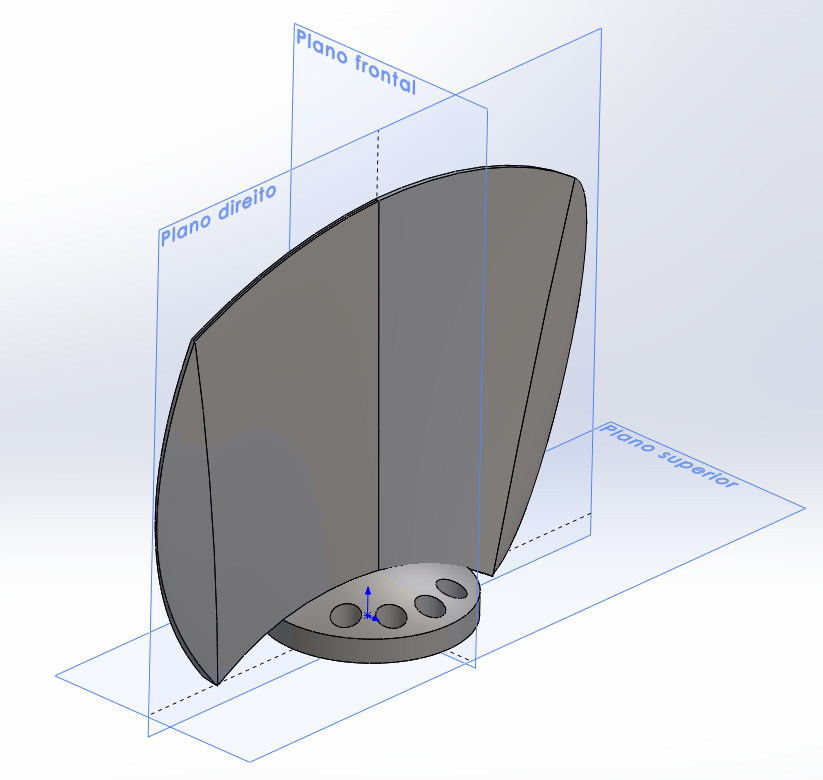
\includegraphics[width=\columnwidth]{figs/bighatch/PaPlanos.PNG}
	\caption{Ilustração das projeções da pá em planos.}
	\label{fig::paplanos}
\end{figure}

\paragraph{KR 10 R1100 sixx WP (Kuka)}
A figura~\ref{fig::kukageom} ilustra a interseção do espaço de trabalho
simplificado do manipulador Kuka KR10 e a projeção da pá. No
caso do Kuka KR 10 R1100, o raio da esfera é aproximado a $\overline{OB^i} = $
alcance do manipulador + comprimento da pistola + 230 mm $= $. 

\begin{figure}[h!]	
	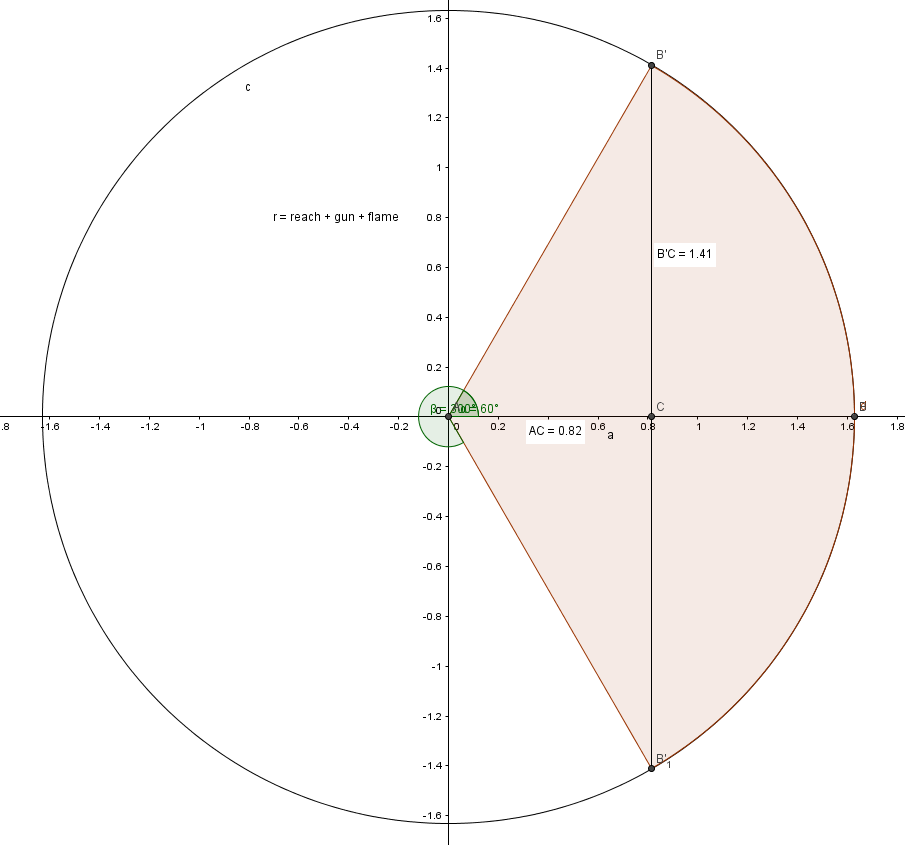
\includegraphics[width=\columnwidth]{figs/bighatch/kukageom.jpg}
	\caption{Ilustração da interseção do espaço de trabalho simplificado do
	manipulador Kuka KR10 e a projeção da pá.}
	\label{fig::kukageom}
\end{figure}

\paragraph{MH12 (Motoman)}

\begin{figure}[h!]	
	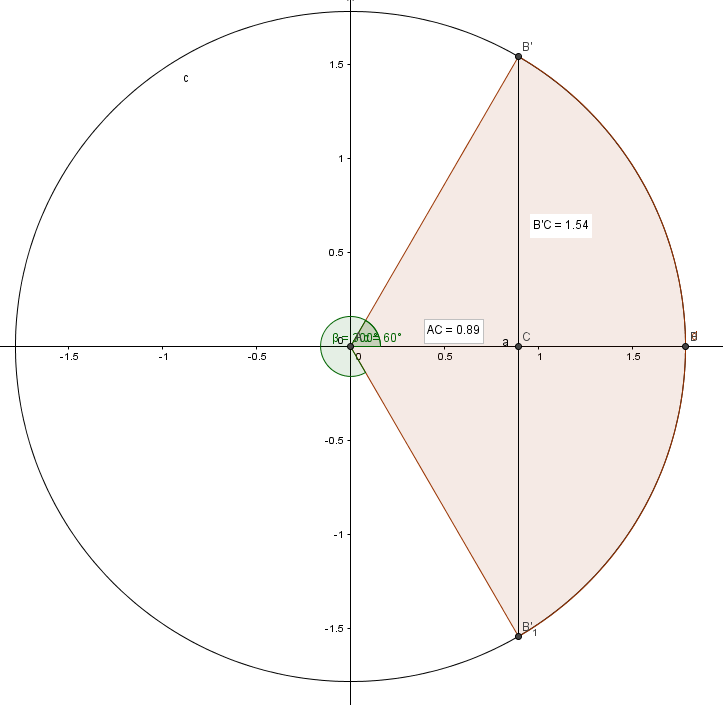
\includegraphics[width=\columnwidth]{figs/bighatch/motomangeom.jpg}
	\caption{Ilustração da interseção do espaço de trabalho simplificado do
	manipulador Motoman MH12 e a projeção da pá.}
	\label{fig::motomangeom}
\end{figure}
\subsubsection{Espaço de trabalho e cinemática do manipulador}
Como já mencionado, o ambiente de simulação foi desenvolvido utilizando a
arquitetura de planejamento Openrave. Para cada manipulador selecionado após a
pesquisa de mercado, serão analisados os reais espaços de trabalho, e o processo de
revestimento da pá em um ambiente simulado que representa as principais
caracterísiticas do ambiente real.

Para gerar o espaço de trabalho, o Openrave utiliza um método de força bruta,
onde são executadas iterações sob iterações de todas as juntas, por seus ângulos
limites e com o passo de ângulo dependendo da resolução do manipulador. O grau
de manipulabilidade do robô é representado por um gradiente de cores, cujo grau
varia do azul claro (menor manipulabilidade) ao vermelho escuro (maior manipulabilidade).
Entende-se por manipulabilidade a capacidade que o robô possui de manipular
objetos em direções específicas, isto é, para uma posição específica é
possível alcançar variadas orientações. Em todas as simulações, a pistola foi
representada como um cilindro de comprimento 300 mm e raio 50 mm, e o efetuador está no extremo do cilindro.

A superfície da pá é amostrada, formando uma grade de tamanho fixo. A técnica
\textit{axis-aligned bounding box (AABB)} é utilizada para obter os
pontos e suas respectivas normais, na superfície da pá. Nesta técnica, a
superfície alvo é inscrita em um bloco, que é uniformemente amostrado. É, então,
realizada uma verificação de colisão entre os pontos amostrados no bloco e a
superfície alvo e, caso haja interseção, o ponto é armazenado junto com sua
normal à superfície. Dessa forma, podemos amostrar a pá e deslocar estes pontos
230 mm em relação à sua normal com a superfície, garantindo a requerimento do
revestimento. A representação dos pontos amostrados e deslocados em relação às
normais da pá podem estão nas figuras~\ref{fig::amostrapa1} e ~\ref{fig::amostrapa2}. 

Utilizando as informações dos pontos amostrados e o espaço de trabalho do
manipulador, foram gerados scripts para calcular a
melhor distância do manipulador em relação a pá, de forma que o maior número de
pontos revestidos com angulação de $90^o$ fossem cobertos.
Essa distância é calculada em relação à normal da pá. Com esse dado, é possível estimar quantas posições da base do
manipulador serão necessários para o revestimento de toda a pá.

\begin{figure}[h!]	
	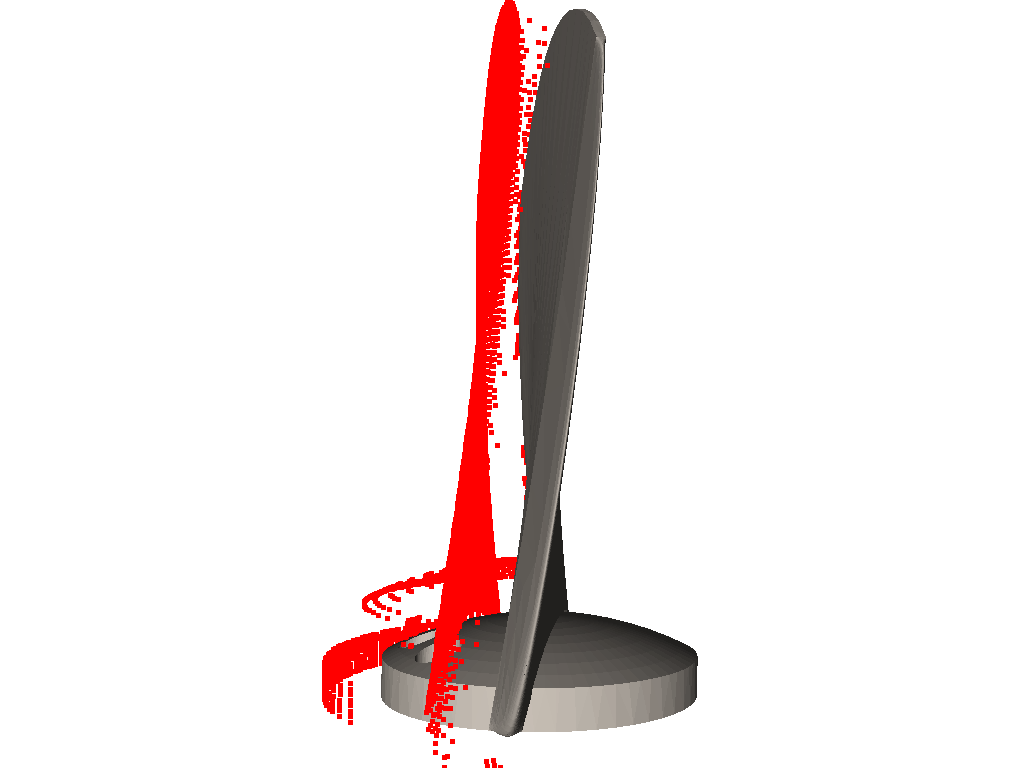
\includegraphics[width=\columnwidth]{figs/bighatch/amostrapa1.png}
	\caption{Pontos amostrados da pá - vista lateral}
	\label{fig::amostrapa1}
\end{figure}

\begin{figure}[h!]	
	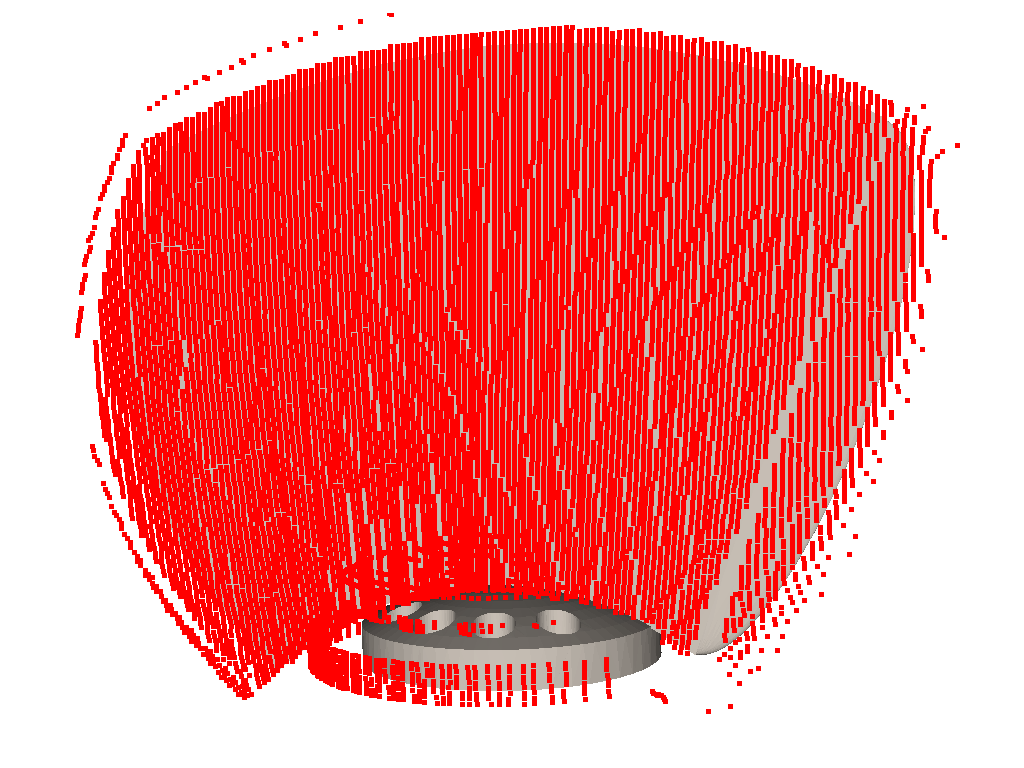
\includegraphics[width=\columnwidth]{figs/bighatch/amostrapa2.png}
	\caption{Pontos amostrados da pá - vista frontal}
	\label{fig::amostrapa2}
\end{figure}

As tabelas~\ref{tab::robocarac} e ~\ref{tab::robocarac} abaixo resume as
caracterísitcas de cada robô e o estudo cinemático realizado, respectivamente:

\begin{center}
\begin{tabular}{  c | c | c | c  }
  \hline
  \textbf{Robô} & \textbf{Payload (Kg)} & \textbf{Massa (Kg)} & \textbf{Alcance
  (mm)} \\ \hline 
  KR10 & 10 & 56 & 1100 \\ \hline
  MH12 & 20 & 130 & 2551  \\ \hline
  LBR 14 & 14 & 30 & 820 \\ \hline
  SIA20D & 20 & 120 &  910 \\
  \hline
\end{tabular}
\captionof{table}{Caracterísitcas principais dos robôs.}
\label{tab::robocarac}
\end{center}

\begin{center}
\begin{tabular}{  c | c | c }
  \hline
  \textbf{Robô} & \textbf{Pontos revestidos (\%)} & \textbf{Posições de base} \\ \hline 
  KR10 & 24.33 & 13\\ \hline 
  MH12 & 53.3 & 4   \\ \hline
  LBR 14 $\uparrow$ & 17.2 & 13 \\ \hline
  LBR 14 $\rightarrow$ & 17.37 & 13 \\ \hline
  SIA20D $\uparrow$ & 23.14 & 9 \\ \hline
  SIA20D $\rightarrow$ & 24.76 & 9 \\ 
  \hline
\end{tabular}
\captionof{table}{Resumo do estudo
cinemático.}
\label{tab::robocin}
\end{center}

\paragraph{KR 10 R1100 sixx WP (Kuka)}
A figura~\ref{fig::kr10cin1} e figura~\ref{fig::kr10cin2} mostram as vistas
lateral e superior do espaço de trabalho do manipulador, respectivamente. Em
vermelho, estão representados os pontos a serem revestidos e em preto os pontos
que o manipulador foi capaz de revestir.

O script que calcula a melhor posição da base em relaçao à pá retornou a posição
870 mm, sendo que 3825 pontos foram revestidos, representando 24.33\% de toda a
pá. Estima-se que serão necessários, pelo menos, 13 posições para o recobrimento
de toda a pá, figura~\ref{fig::kr10bestpos}.



\begin{figure}[h!]	
	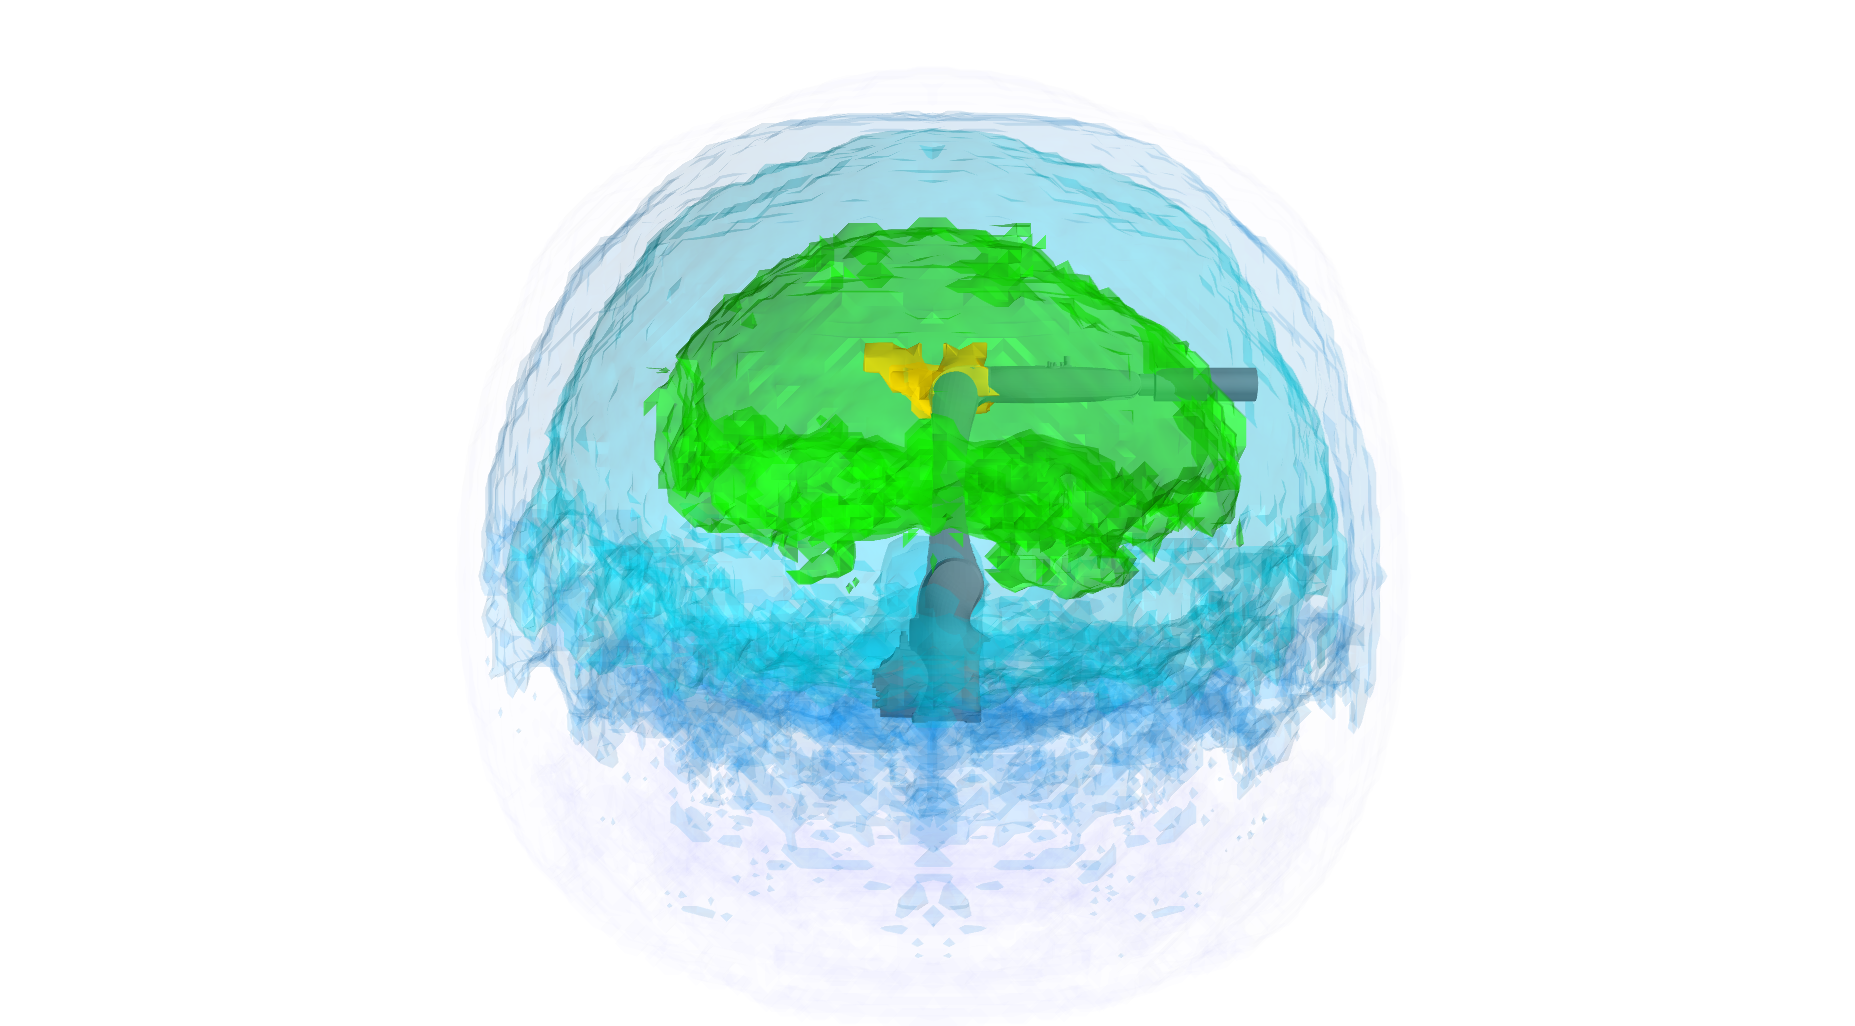
\includegraphics[width=\columnwidth]{figs/bighatch/kr10_front.png}
	\caption{Espaço de trabalho do manipulador Kuka KR10 - vista lateral}
	\label{fig::kr10cin1}
\end{figure}

\begin{figure}[h!]	
	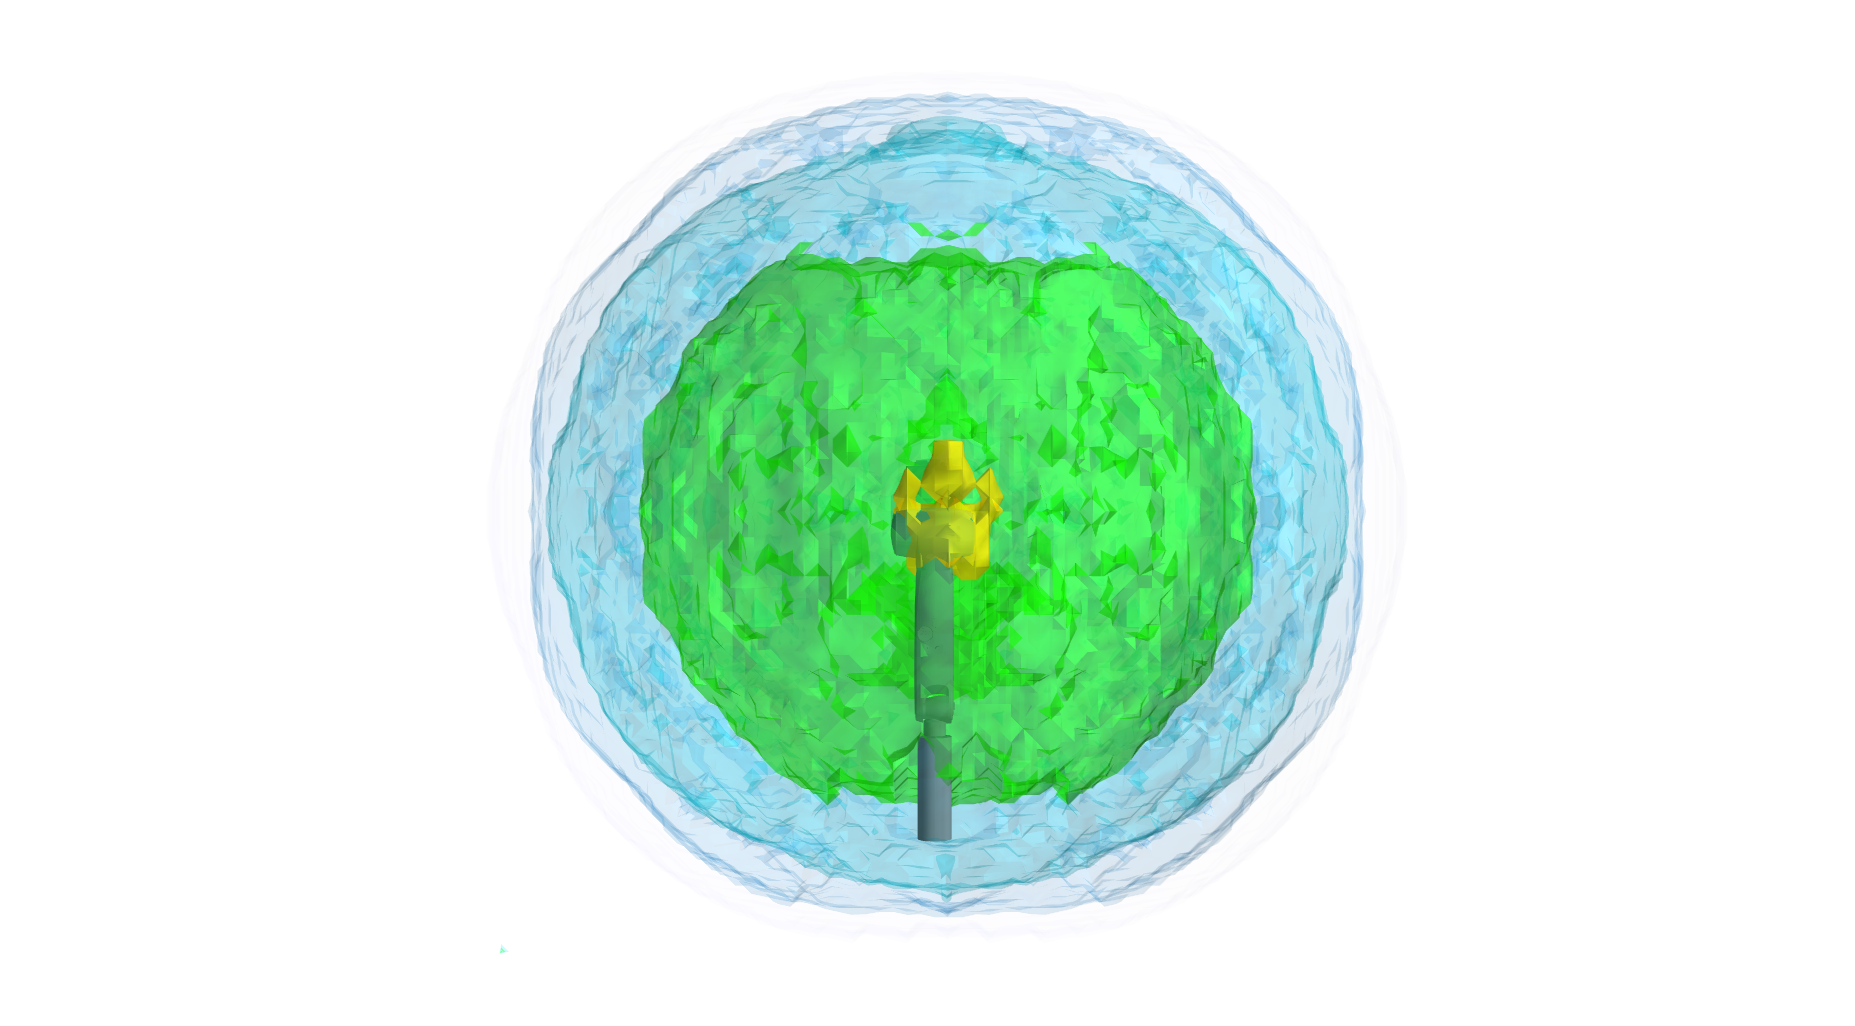
\includegraphics[width=\columnwidth]{figs/bighatch/kr10_top.png}
	\caption{Espaço de trabalho do manipulador Kuka KR10 - vista superior}
	\label{fig::kr10cin2}
\end{figure}

\begin{figure}[h!]	
	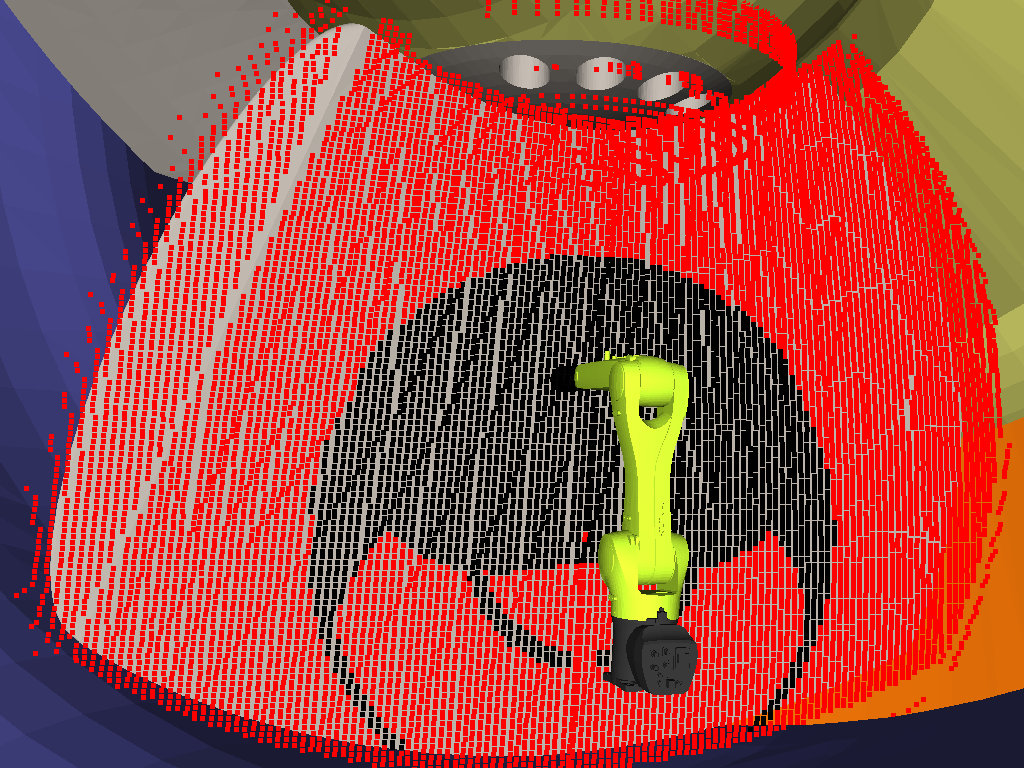
\includegraphics[width=\columnwidth]{figs/bighatch/kr10_bestpos.png}
	\caption{Melhor posição para o revestimento - robô KR10 da Kuka.}
	\label{fig::kr10bestpos}
\end{figure}


\paragraph{MH12 (Motoman)}
A figura~\ref{fig::mh12cin1} e figura~\ref{fig::mh12cin2} mostram as vistas
lateral e superior do espaço de trabalho do manipulador, respectivamente.

O script que calcula a melhor posição da base em relaçao à pá retornou a posição
950 mm, sendo que 8379 pontos foram revestidos, representando 53.30\% de toda a
pá. Estima-se que serão necessários, pelo menos, 4 posições para o recobrimento
de toda a pá, figura~\ref{fig::mh12bestpos}.

\begin{figure}[h!]	
	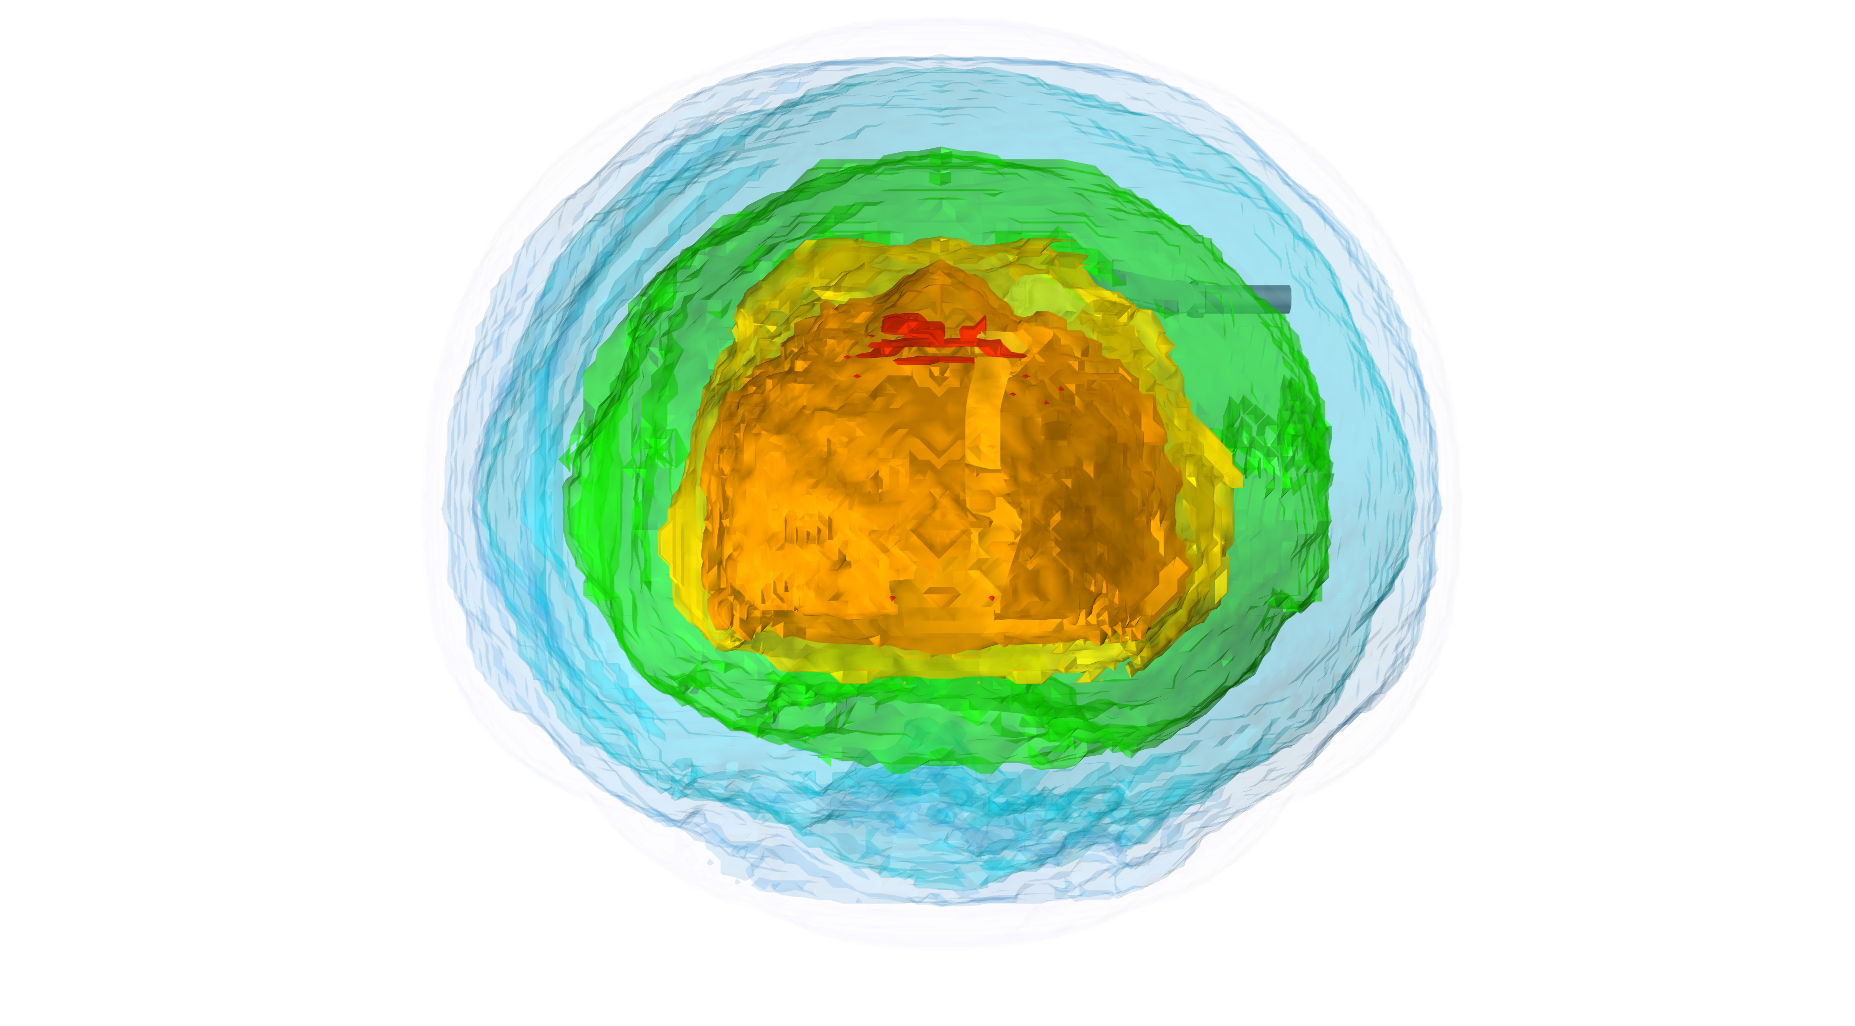
\includegraphics[width=\columnwidth]{figs/bighatch/mh12_front.png}
	\caption{Espaço de trabalho do manipulador MH12 - vista lateral}
	\label{fig::mh12cin1}
\end{figure}

\begin{figure}[h!]	
	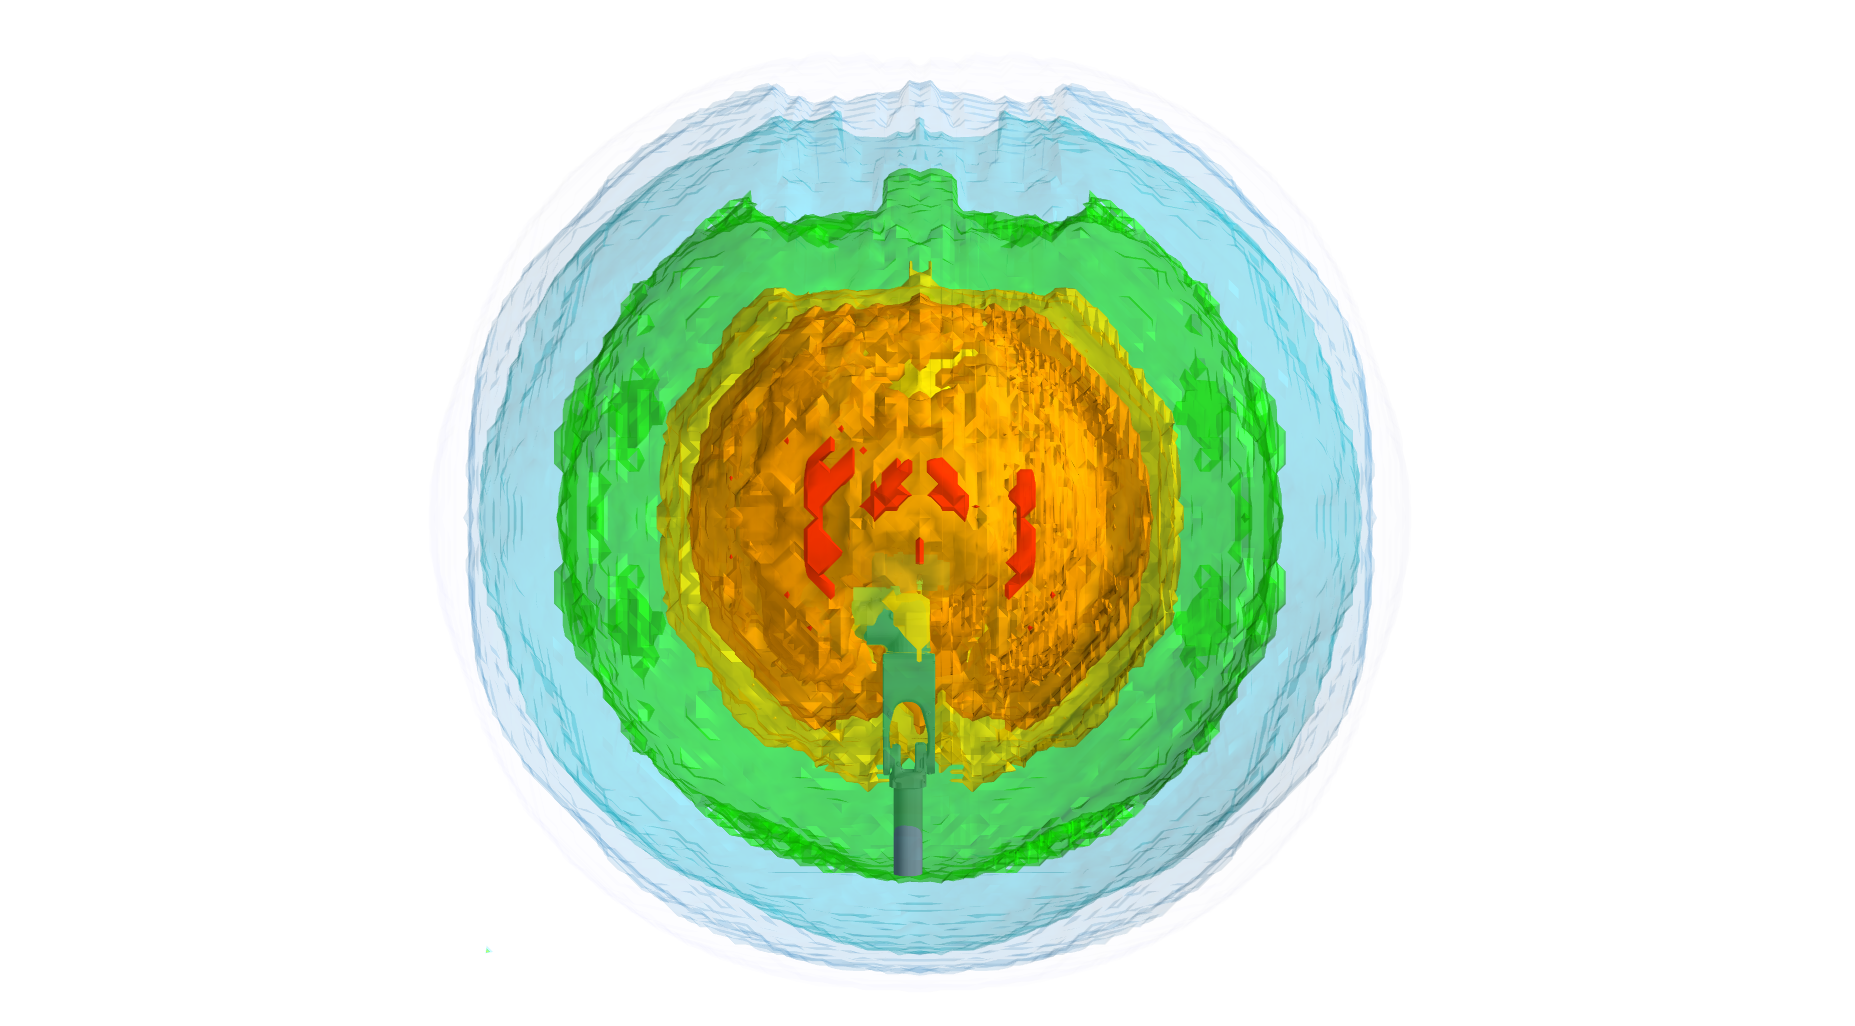
\includegraphics[width=\columnwidth]{figs/bighatch/mh12_top.png}
	\caption{Espaço de trabalho do manipulador MH12 - vista superior}
	\label{fig::mh12cin2}
\end{figure}

\begin{figure}[h!]	
	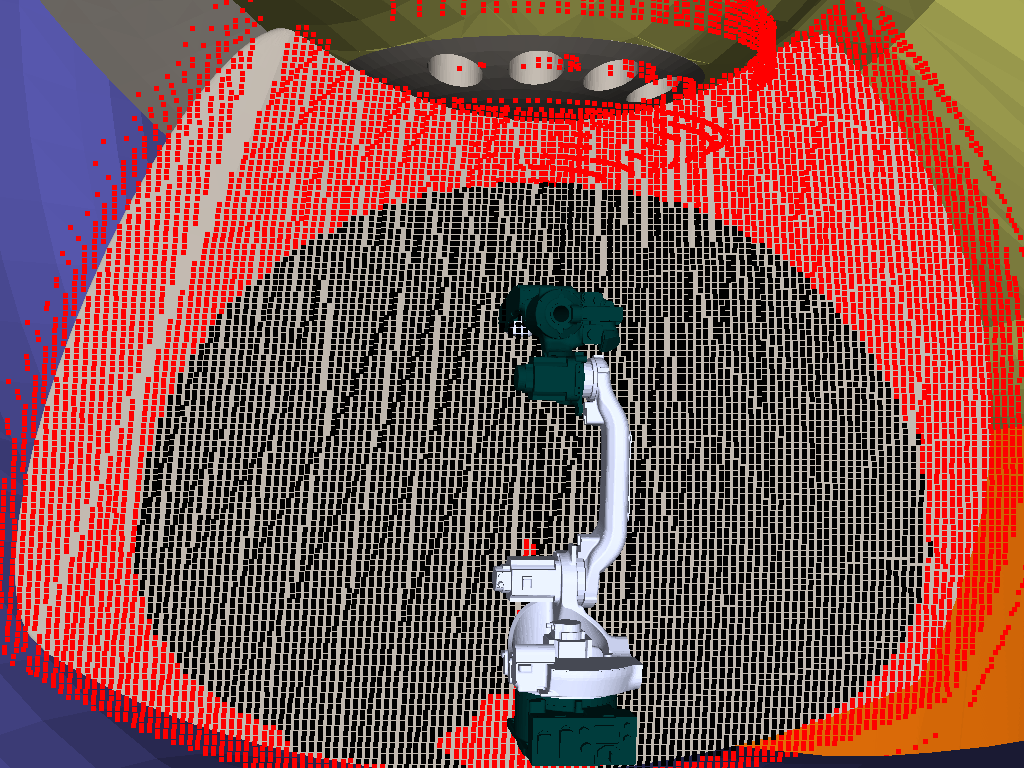
\includegraphics[width=\columnwidth]{figs/bighatch/mh12_bestpos.png}
	\caption{Melhor posição para o revestimento - robô MH12 da Motoman.}
	\label{fig::mh12bestpos}
\end{figure}


\paragraph{LBR iiwa 14 R820 (Kuka)}
O manipulador LBR iiwa 14 R820 possui 7 graus de liberdade e, devido a sua
grande flexibilidade e facilidade de montagem, foram estudadas duas
configurações para a base.

O script que calcula a melhor posição da base na posição vertical em relaçao à
pá retornou a posição 1.06, sendo que 2648 pontos foram revestidos,
representando 17.20\% de toda a pá. Estima-se que serão necessários, pelo menos,
13 posições para o recobrimento de toda a pá, figura~\ref{fig::lbrbestposv}.

\begin{figure}[h!]	
	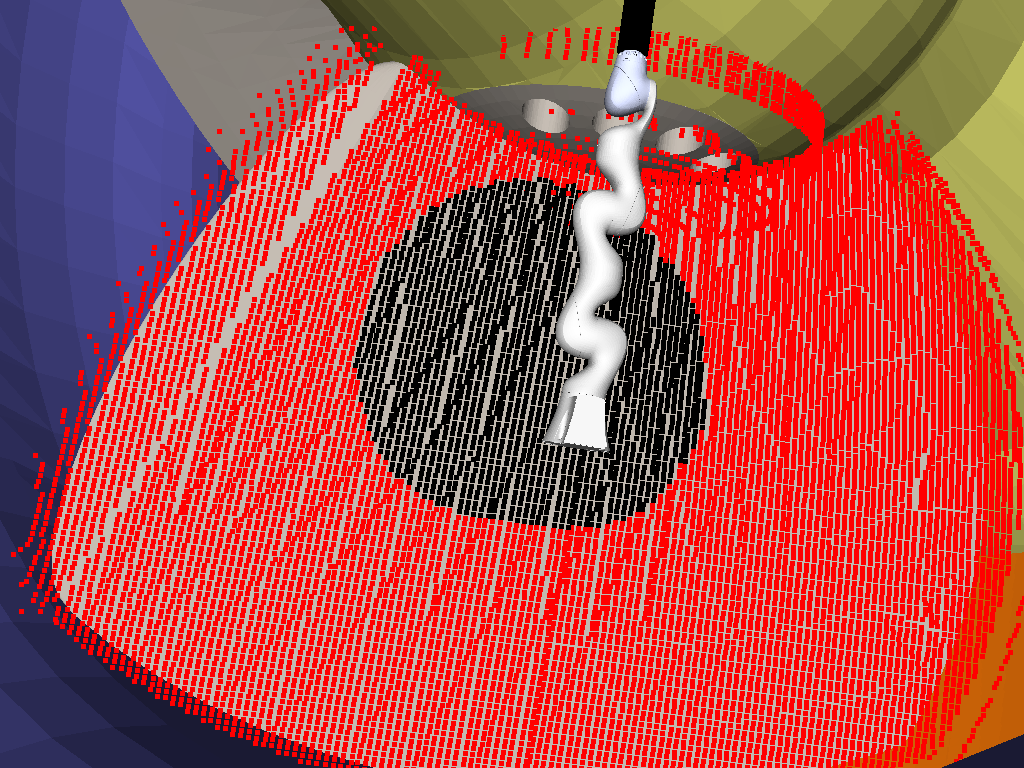
\includegraphics[width=\columnwidth]{figs/bighatch/lbr_bestposv.png}
	\caption{Melhor posição para o revestimento - robô LBR da Kuka com base na
	posição vertical.}
	\label{fig::lbrbestposv}
\end{figure}

O script que calcula a melhor posição da base na posição vertical em relaçao à
pá retornou a posição 1400 mm, sendo que 2730 pontos foram revestidos,
representando 17.37\% de toda a pá. Estima-se que serão necessários, pelo menos,
13 posições para o recobrimento de toda a pá, figura~\ref{fig::lbrbestposh}.

\begin{figure}[h!]	
	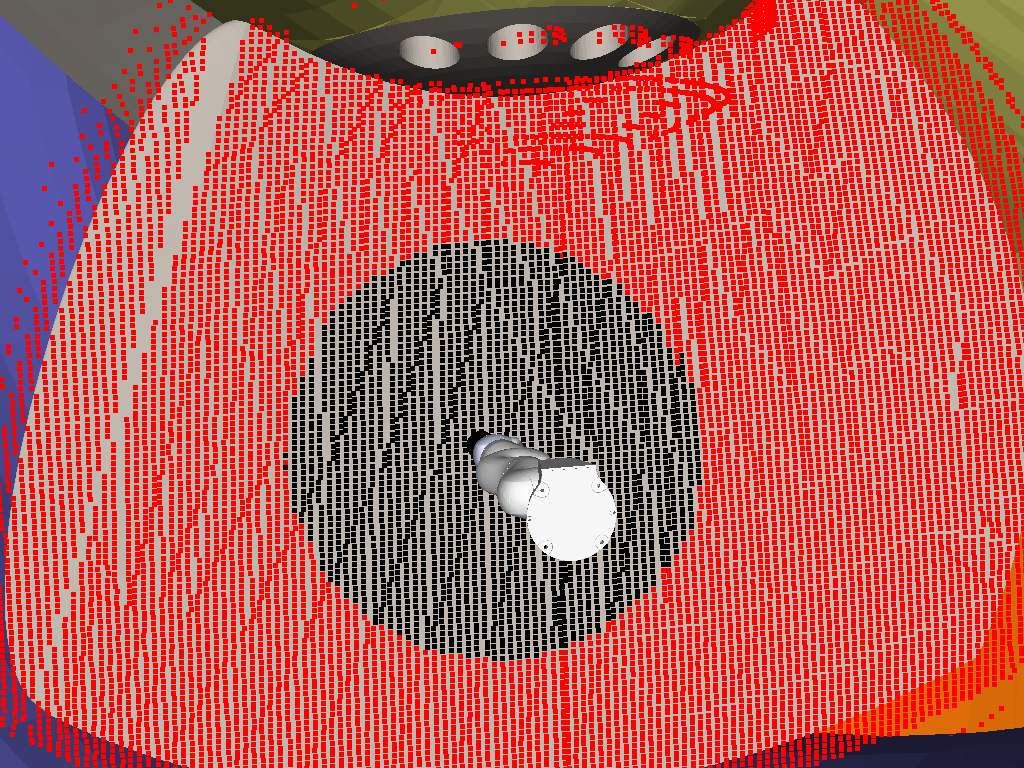
\includegraphics[width=\columnwidth]{figs/bighatch/lbr_bestposh.png}
	\caption{Melhor posição para o revestimento - robô LBR da Kuka com base na
	posição horizontal.}
	\label{fig::lbrbestposh}
\end{figure}

\paragraph{SIA20D (Motoman)}
O manipulador SIA20D também possui 7 graus de liberdade e, devido a sua
grande flexibilidade e facilidade de montagem, foram estudadas duas
configurações para a base.

O script que calcula a melhor posição da base na posição vertical em relaçao à
pá retornou a posição 1100 mm, sendo que 3638 pontos foram revestidos,
representando 23.14\% de toda a pá. Estima-se que serão necessários, pelo menos,
9 posições para o recobrimento de toda a pá, figura~\ref{fig::sia20dbestposv}.

\begin{figure}[h!]	
	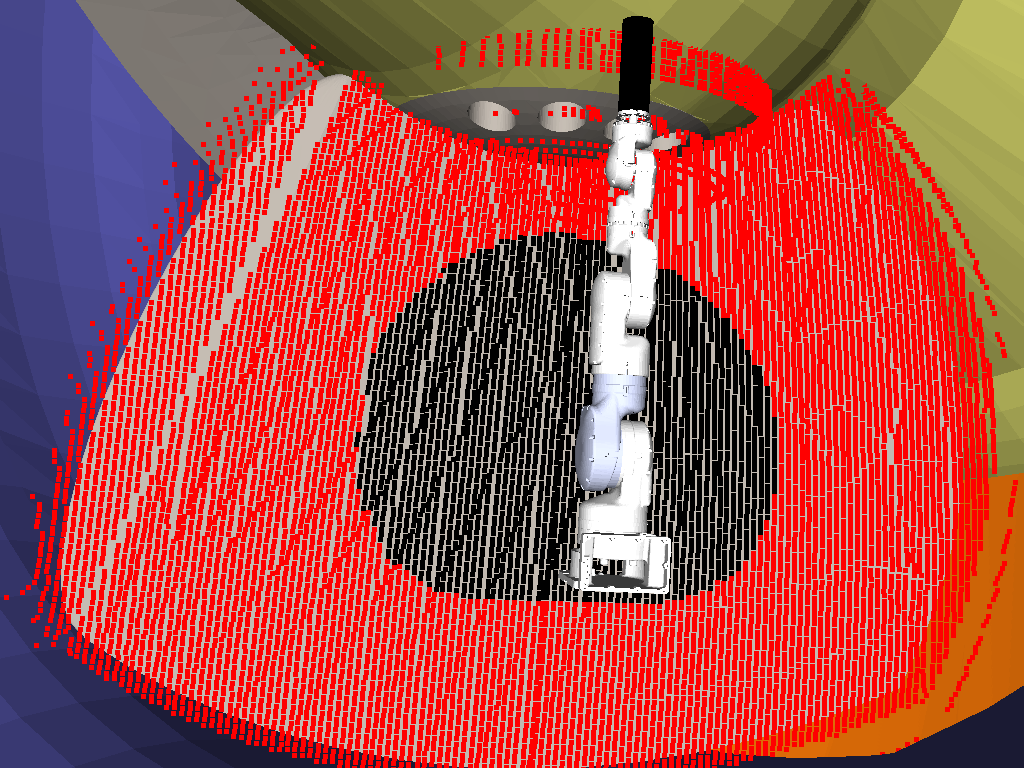
\includegraphics[width=\columnwidth]{figs/bighatch/sia20d_bestposv.png}
	\caption{Melhor posição para o revestimento - robô SIA20D da Motoman com base
	na posição vertical.}
	\label{fig::sia20dbestposv}
\end{figure}

O script que calcula a melhor posição da base na posição horizontal em relaçao à
pá retornou a posição 1510 mm, sendo que 3892 pontos foram revestidos,
representando 24.76\% de toda a pá. Estima-se que serão necessários, pelo menos,
9 posições para o recobrimento de toda a pá, figura~\ref{fig::sia20dbestposh}.

\begin{figure}[h!]	
	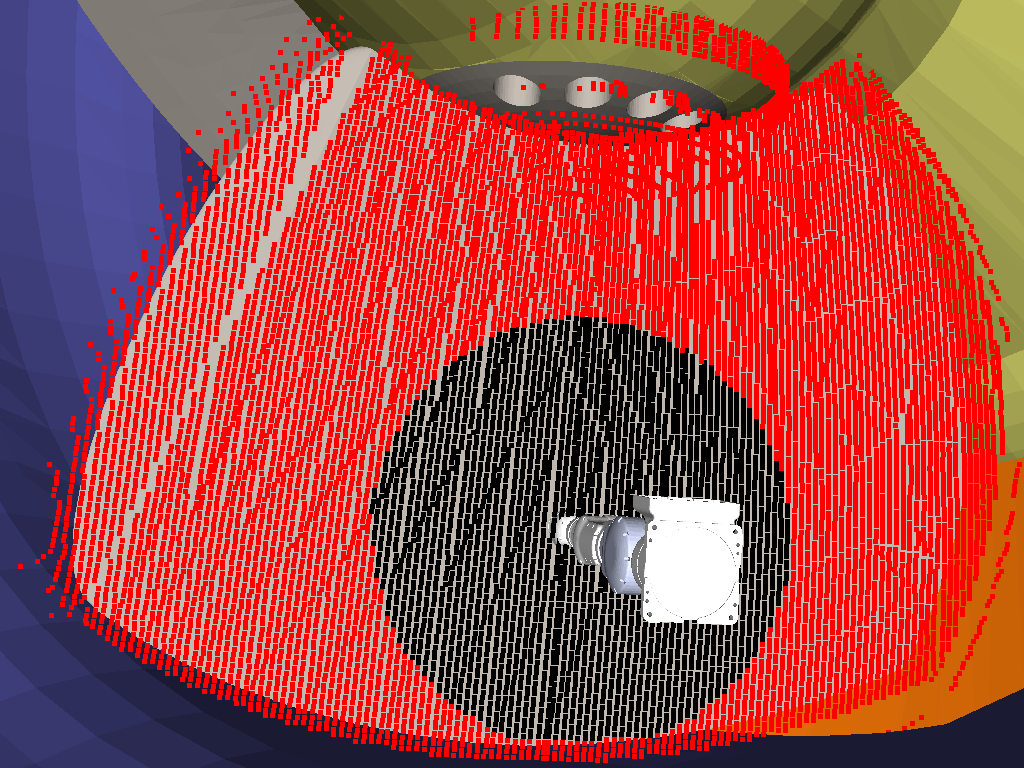
\includegraphics[width=\columnwidth]{figs/bighatch/sia20d_bestposh.png}
	\caption{Melhor posição para o revestimento - robô SIA20D da Motoman com base
	na posição horizontal.}
	\label{fig::sia20dbestposh}
\end{figure}

\paragraph{Tolerância no ângulo de revestimento}
As análises de revestimento dos manipuladores exigiram que a pistola
estivesse com as mesmas direções e sentidos opostos às normais dos
pontos a serem revestidos, isto é, a orientação da pistola é sempre
perpendicular ao plano da pá. Entretanto, pode-se assumir uma tolerância de
$90^o \pm 60^o$ entre a pistola e o plano perpendicular, que foi considerada
na análise puramente geométrica. Como o manipulador MH12 (Motoman) possui
recobrimento de quase todo o alcance vertical da pá (revestimento de cima a
baixo), mostra-se interressante a análise de tolerância neste manipulador, de
forma que haja simplificação das possíveis soluções de bases.

Primeiramente, são armazenados os pontos que o robô não foi capaz de
revestir (pontos em vermelho, nas figuras de espaço de trabalho dos
manipuladores) e suas respectivas normais aos planos tangentes à superfície da
pá. Os pontos são deslocados 230 mm na mesma direção e sentido oposto às suas
respectivas normais, de forma que pertençam à superfície da pá,
ponto $D$ é deslocado até ponto $C$ na figura~\ref{fig::tolerancia1}. Para cada
ponto não revestido, são gerados dois vetores unitários $\overrightarrow{v}$ e
$\overrightarrow{w}$ ortogonais entre si e ao vetor normal $\overrightarrow{N}$,
no plano tangente à superfície da pá conforme
ilustrado na figura~\ref{fig::tolerancia2}. O vetor $\overrightarrow{N}$ é
girado pelo ângulo de tolerância de revestimento $\theta$ (entre $0^o$ e $60^o$)
em relação ao vetor $\overrightarrow{w}$, gerando o vetor
$\overrightarrow{P_1}$, figura~\ref{fig::tolerancia3}.

\begin{figure}[h!]	
	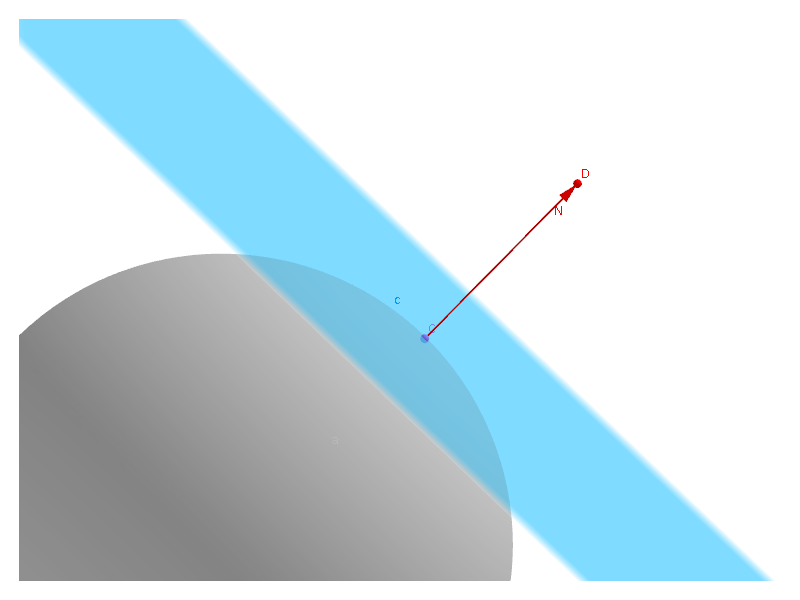
\includegraphics[width=\columnwidth]{figs/bighatch/tolerancia1.png}
	\caption{Ponto D não revestido, deslocado 230 mm da superfície da pá.}
	\label{fig::tolerancia1}
\end{figure}

\begin{figure}[h!]	
	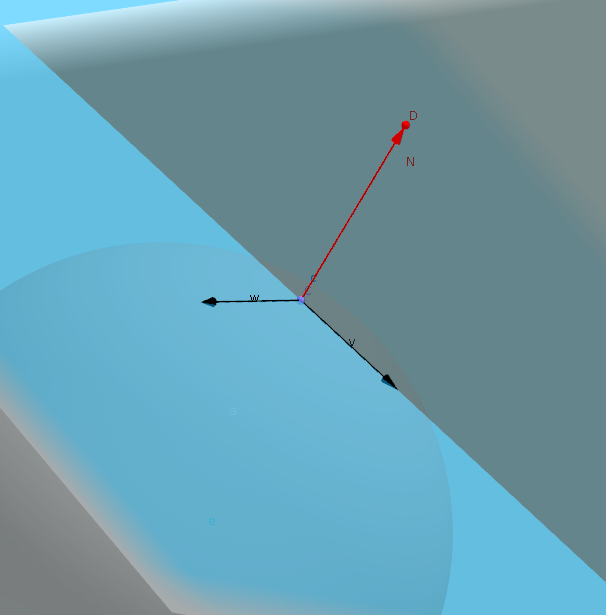
\includegraphics[width=\columnwidth]{figs/bighatch/tolerancia2.png}
	\caption{Vetores v e w ortogonais ao vetor normal N.}
	\label{fig::tolerancia2}
\end{figure}

Finalmente, o vetor $\overrightarrow{P_1}$ pode ser girado em relação a
$\overrightarrow{N}$ e todos os vetores que pertencem à tolerância de
revestimento $\theta$ saem do ponto $C$ até um ponto do círculo $h$, como o
vetor exemplo $\overrightarrow{P_2}$, na figura~\ref{fig::tolerancia4}. Observe
que este círculo deve ser discretizado, e cada ponto pertencente ao círculo e sua
respectiva normal (vetor de origem $C$ ao ponto do círculo) devem ser
reavaliados, isto é, verifica-se se o robô alcança o ponto pertencente a $h$ com
pistola de revestivemto apontada a sua respectiva normal.
Se algum ponto do círculo puder ser revestido, o ponto $D$ pode ser considerado
como revestido. No exemplo da figura~\ref{fig::tolerancia4}, o círculo $h$ foi
discretizado em dois pontos $G$ e $H$, e suas normais são $\overrightarrow{P_1}$
e $\overrightarrow{P_2}$, respectivamente. 

\begin{figure}[h!]	
	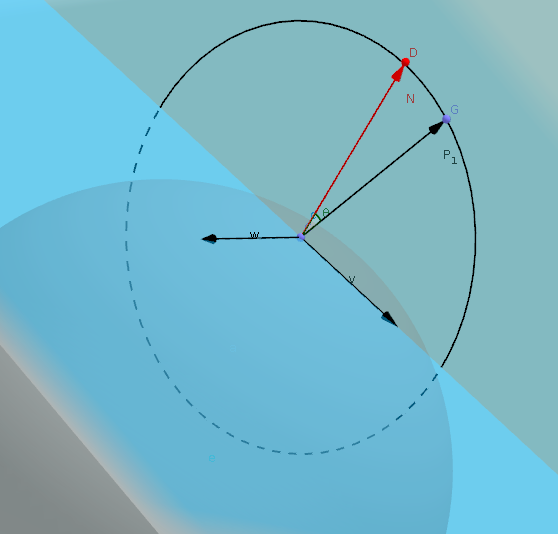
\includegraphics[width=\columnwidth]{figs/bighatch/tolerancia3.png}
	\caption{Vetor N girado pelo ângulo de tolerância de revestimento.}
	\label{fig::tolerancia3}
\end{figure}

\begin{figure}[h!]	
	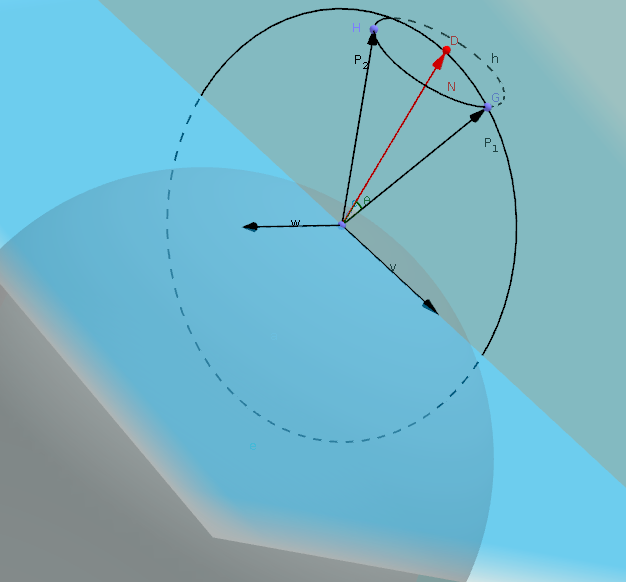
\includegraphics[width=\columnwidth]{figs/bighatch/tolerancia4.png}
	\caption{Circulo $h$ representa todos os pontos equivalentes ao ponto $D$ com
	ângulo de tolerância de revestimento $\theta$.}
	\label{fig::tolerancia4}
\end{figure}

Foram realizadas análises de tolerância para dois robôs: MH12, que apresentou o
maior número de pontos revestido na pá, e LBR R820, que é a única solução viável
de manipulador industrial para o acesso superior. Os ângulos de tolerância foram
variados em $10^o$ e $30^o$. 

\subsubsection{Dinâmica do manipulador}
A dinâmica de um manipulador robótico é a análise de velocidades, acelerações e
torques das juntas. Para esta análise, assume-se que o efetuador, pistola de
revestimento, possui velocidade 40m/min constante em todos os pontos amostrados
da pá. Como velocidades e acelerações exigem a computação de derivadas, é
realizada uma melhor discretização da pá da turbina, na qual o passo de
amostragem é menor e um filtro garante espaçamento uniforme dos pontos de 10 mm.
Para um lado da pá, são amostrados, portanto, 130 mil pontos.

Para cada ponto amostrado da pá, faz-se a análise cinemática e são armazenados
os pontos que são possíveis de serem revestidos, como na
seção~\ref{sec::cinematica}, isto é, são armazenados os pontos que possuem
solução de cinemática inversa. Posteriormente, para cada ponto revestido, é
criado um conjunto contendo seus 8 pontos vizinhos através de um algoritmo k-d
tree, como na figura~\ref{fig::pontosdin}, onde $p_r$ é o ponto de referência a
ser analisado dinamicamente e os pontos ${p_1,p_2,q_1,q_2,r_1,r_2,s_1,s_2}$ são auxiliares
para o estudo. 

\begin{figure}[h!]	
	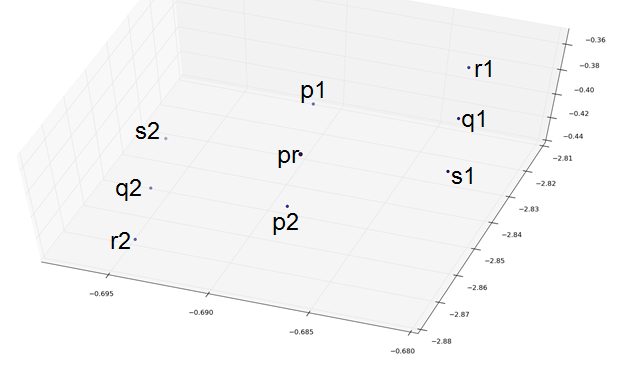
\includegraphics[width=\columnwidth]{figs/dinamica/pontosdinamica.png}
	\caption{Pontos exemplo amostrados da pá.}
	\label{fig::pontosdin}
\end{figure}

%As soluções de cinemática inversa (ângulos das juntas do robô)
%$\Theta_r
%=
%{\theta_{p_r},\theta_{p_1},\theta_{p_2},\theta_{q_1},\theta_{q_2},\theta_{r_1},\theta_{r_2},\theta_{s_1},\theta_{s_2}}$
As velocidades angulares das juntas são calculadas a partir da cinemática
diferencial. Para isso, usa-se o cálculo da matriz jacobiana ($J$), que é a
diferenciação (derivadas parciais) da matriz de cinemática direta em função das
variáveis de junta \citep{sciavicco2000differential}. A velocidade linear do
efetuador ($\dot{X}$) e o jacobiano são conhecidos em cada ponto de referência, logo
podem-se calcular as velocidades das juntas do manipulador entre o ponto de
referência e cada ponto auxiliar: $\dot{X} = J\dot{q}\Rightarrow
J^+\dot{X}=\dot{q}$, onde $J^+$ é a pseudo inversa Moore-Penrose de $J$.

As velocidades angulares são $\Omega_r
=
\{\omega_{p_r,p_1},\omega_{p_r,p_2},\omega_{p_r,q_1},\omega_{p_r,q_2},\omega_{p_r,r_1},\omega_{p_r,r_2},\omega_{p_r,s_1},\omega_{p_r,s_2}\}$,
onde $\omega$, $\omega\in\Omega_r$, é um vetor $n \times 1$, e $n$ é o número de
juntas do robô. As velocidades dos ângulos das juntas é uma informação importate para a
verificação da viabilidade das trajetórias do robô. Para o caso do robô
MH12, onde $\omega_{\textbf{max}}=\{220, 200, 220, 410, 410, 610\}^o/s$, por
exemplo, caso não haja $\omega\in\Omega_r$, tal que
$\omega\leq\omega_{\textbf{max}}$, não é possível realizar o revestimento do
ponto de referência $p_r$. Se $\exists \omega\in\Omega_r$ tal que
$\omega\leq\omega_{\textbf{max}}$, o ponto de referência é viável pela
cinemática inversa e pela cinemática diferencial, mas pode ser inviável ainda
pela análise dinâmica, que considera as acelerações, massas e forças do
conjunto.

As equações dinâmicas de um manipulador são também abordados em
\cite{sciavicco2000differential} e possuem duas abordagens bem conhecidas na
literatura: equações de Newton-Euler e equações de Lagrange. O ambiente OpenRave
utiliza o método de Newton-Euler para computar os torques das juntas (dinâmica
inversa): $\tau = M(q)\alpha + C(q,\omega)\omega + G(q) $, onde $\tau$ é o
vetor de torques das juntas, $M$ matriz de massas e momentos de inércia,
$\alpha$ é acelerações das juntas, $C$ matriz de Coriolis, $\omega$ é as
velocidades das juntas e $G$ o vetor de gravidade.

Para a formação da matriz $M$, é necessária a estimação de parâmetros do
manipulador. A estimação dos parâmetros pode ser realizada de maneira iterativa,
isto é, aplicam-se torques nas juntas e, pela resposta
do manipulador, estima-se a matriz \citep{slotine1988adaptive}; ou pelo CAD do
manipulador, por exemplo, pela utilização da ferramenta SolidWorks. Foi utilizado o método de estimação pelo CAD do
manipulador, visto que os manipuladores ainda estavam em estudo e não foram
adquiridos, além disso houve facilidade de aproximar os parâmetros já que o CAD
fornecido pelo fabricante é bem detalhado. 

A aceleração angular, $\alpha$, é necessária para a computação dos torques,
$\tau$. O método analítico para cálculo da aceleração angular das juntas é
através da derivada da equação da cinemática diferencial:
$\ddot{X}=\dot{q}^TH\dot{q}+J\ddot{q} \Rightarrow
\ddot{q}=J^+(\ddot{X}-\dot{q}^TH\dot{q})$ ou
$\alpha=J^+(a-\omega^TH\omega)$, onde $H$ é a matriz Hessiana, isto é, derivada
parcial da matriz jacobiana $J$ \citep{hourtash2005kinematic}. 

Com a informação dos ângulos, velocidades e acelerações das juntas, momentos
de inércia e massa dos elos, o OpenRave calcula a dinâmica inversa através do
método Newton-Euler, obtendo-se os torques. Para cada ponto de referência, há quatro direções
(trajetórias) possíveis amostradas que o efetuador pode percorrer:
$\{(p_1,p_r,p_2),(q_1,p_r,q_2),(r_1,p_r,r_2),(s_1,p_r,s_2)\}$, logo quatro
ângulos, velocidades e acelerações de juntas, portanto são obtidos quatro
possíveis vetores de torques:
$T=\{\tau_{rp},\tau_{rq},\tau_{rr},\tau_{rs}\}$. E, especificamente para o
caso do manipulador MH12, os valores dos torques devem ser inferiores aos
estabelecidos pelo datasheet:
$\tau_{\textbf{max}}=\{-,-,-,22,22,9.8\}\textbf{Nm}$, logo se $\exists \tau\in
T$, tal que $\tau\leq\tau_{\textbf{max}}$, então há uma trajetória viável.

As figuras~\ref{fig::wgeo}, ~\ref{fig::wcin} e ~\ref{fig::wdin} representam a
evolução das análises do manipulador, de um nível mais simples a um nível mais
complexo de detalhamento, o qual avalia velocidades, acelerações e torques das
juntas do manipulador. Ainda deverá ser executada a análise de manipulabilidade
que avalia o sistema de controle do manipulador. Esta análise é importante para
o planejamento de trajetórias do manipulador e para o cálculo das posições
viáveis da base para uma operação completa.



\begin{figure}[h!]	
	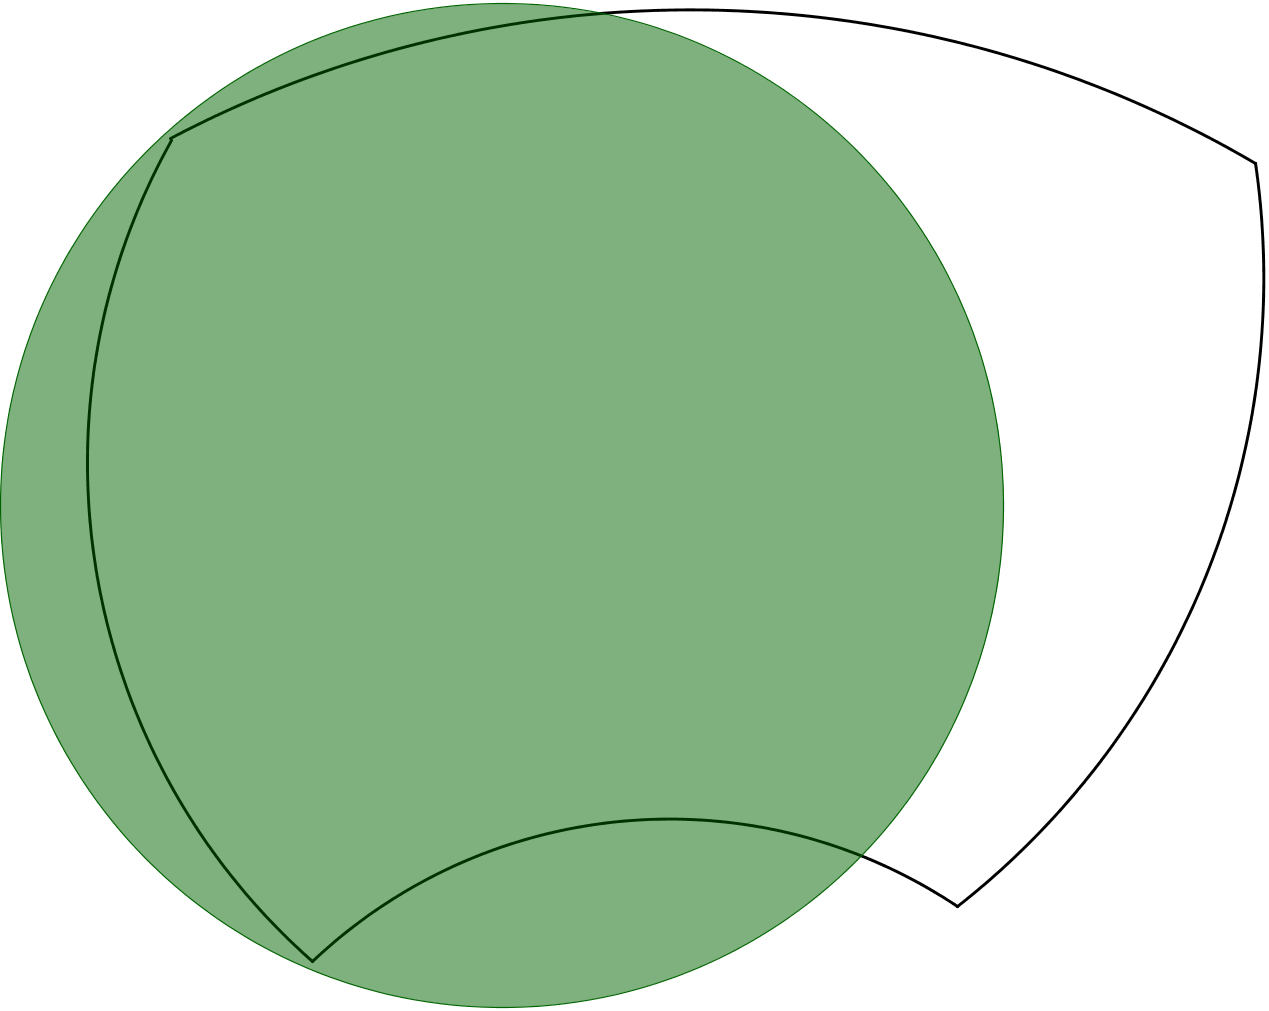
\includegraphics[width=\columnwidth]{figs/dinamica/workspaceGeometrico.png}
	\caption{Área em verde representa a cobertura do revestimento executada pelo
	manipulador, utilizando a abordagem puramente geométrica.}
	\label{fig::wgeo}
\end{figure}

\begin{figure}[h!]	
	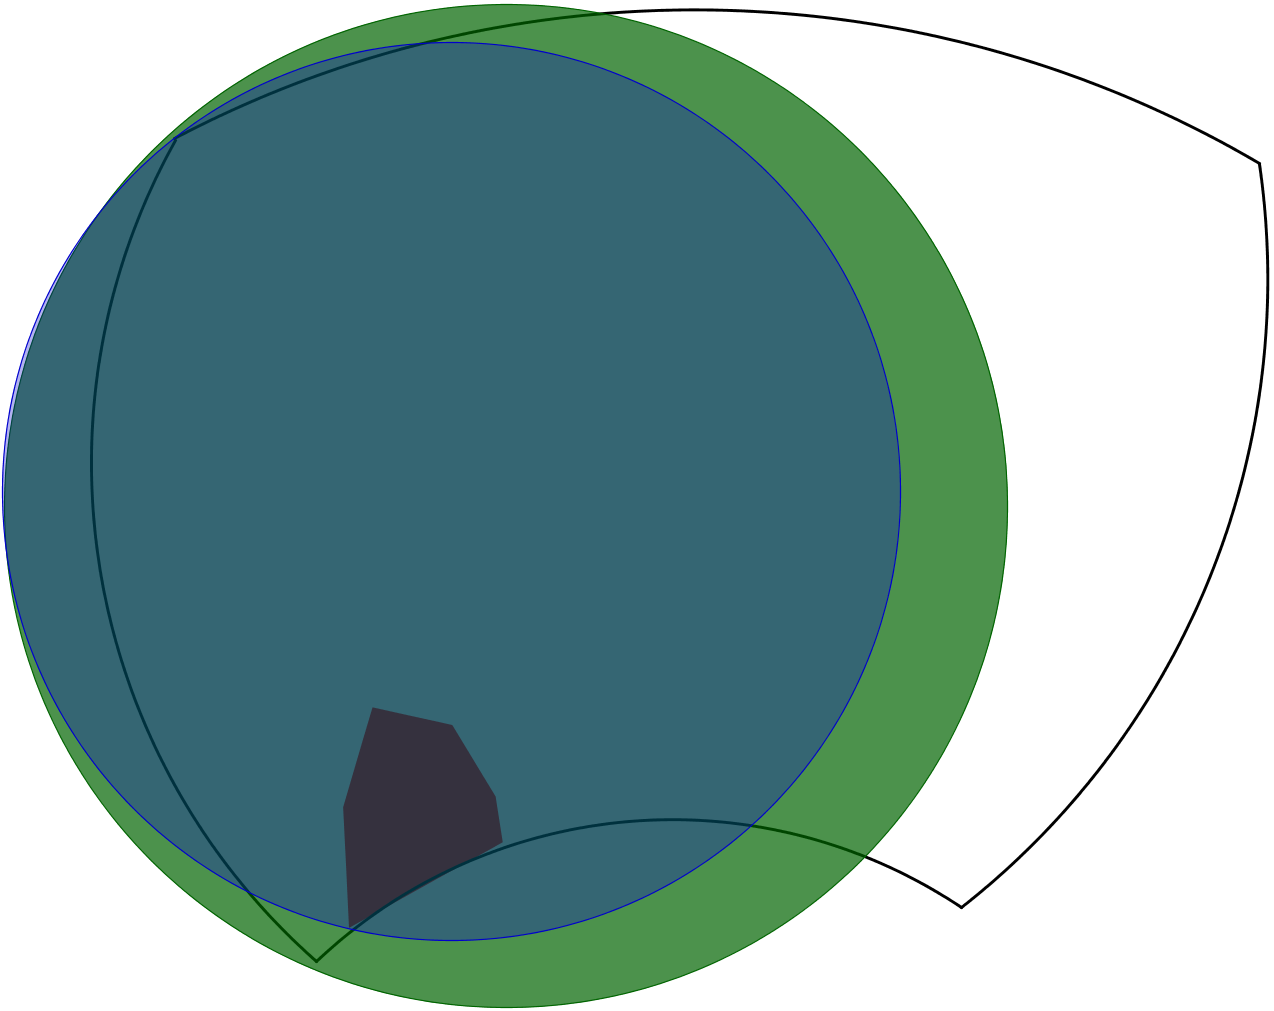
\includegraphics[width=\columnwidth]{figs/dinamica/workspaceCinematica.png}
	\caption{Área em verde representa a cobertura do revestimento executada pelo
	manipulador, utilizando a abordagem puramente cinemática.}
	\label{fig::wcin}
\end{figure}

\begin{figure}[h!]	
	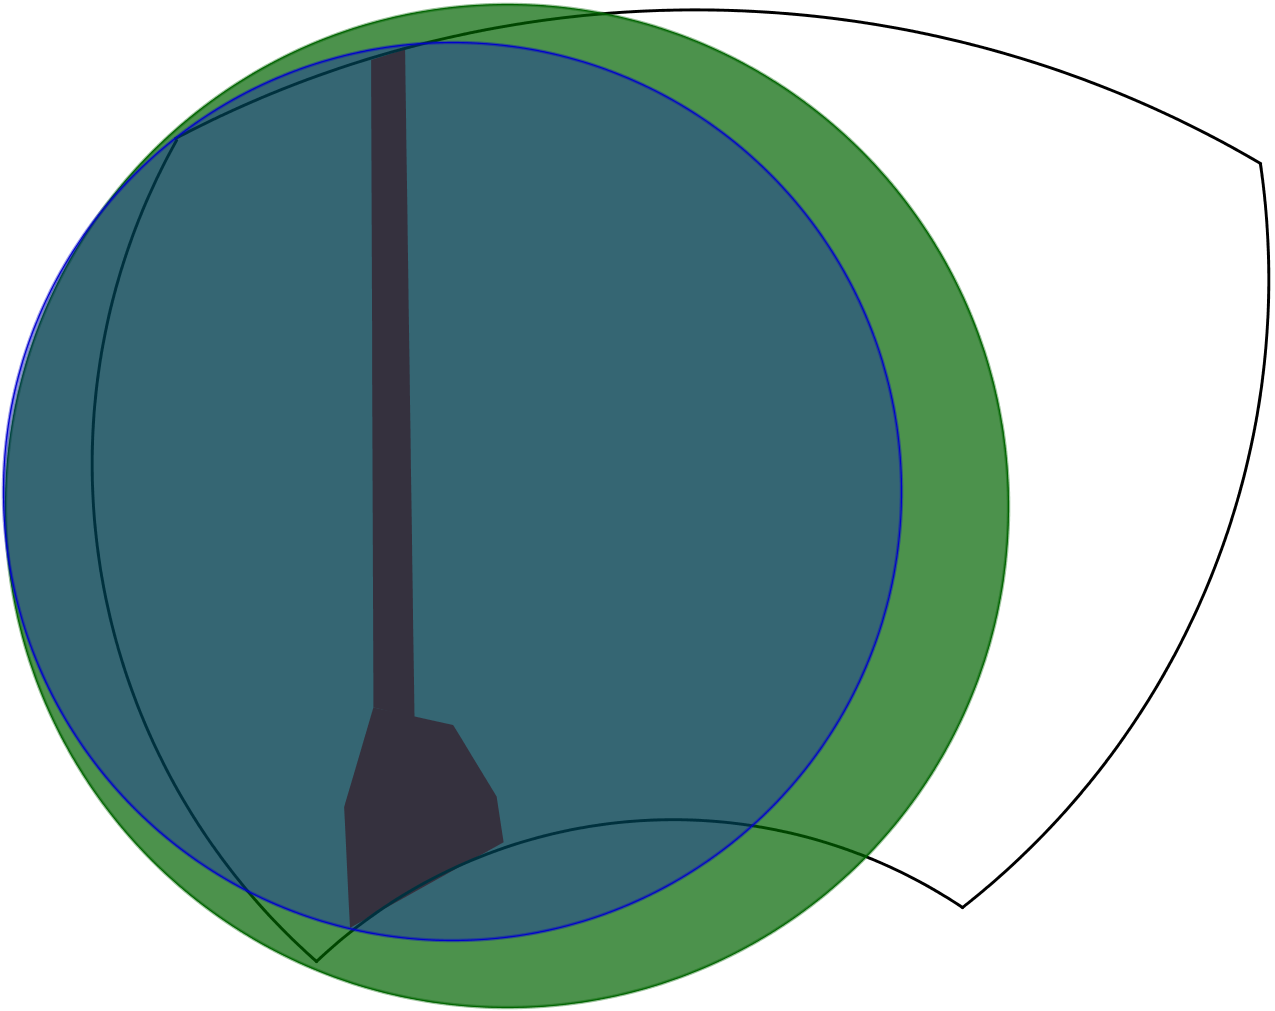
\includegraphics[width=\columnwidth]{figs/dinamica/workspaceTorques.png}
	\caption{Área em verde representa a cobertura do revestimento executada pelo
	manipulador, utilizando a abordagem dinâmica.}
	\label{fig::wdin}
\end{figure}
\subsubsection{Detalhamento da Base Mecânica}\label{sec::base_mec}
A base mecânica é composta pelos elementos de suporte, transporte e ancoragem do
robô no interior da turbina. Os elementos de suporte formam a estrutura
principal da base, que estruturam o ambiente para a montagem, movimentação e
funcionamento seguros do robô. Os elementos de transporte oferecem ao
manipulador graus de liberdade que permitem que este se posicione com facilidade
nos pontos ótimos para o processo. Estes elementos podem ser trilhos, atuadores
lineares, mancais de rolamento, atuadores rotativos, etc. Os elementos de
ancoragem são necessários para fixar o robô e a estrutura no ambiente. As
opções de ancoragem estudadas foram as bases magnéticas e solda, sendo a
primeira opção de preferência pois há menor risco de danificar o ambiente. As
etapas de detalhamento da base mecânica seguem a seguinte ordem: $1)$ investigação dos
graus de liberdade necessários; $2)$ configuração conceitual da base em função
dos graus de liberdade; $3)$ escolha do melhor conceito; $4)$ escolha e
dimensionamento dos elementos mecânicos que compõem a base; $5)$ testes.
Avaliamos até esta etapa do projeto os itens: $1$,$2$ e $3$.

Os graus de liberdade são fornecidos através de combinações de juntas
prismáticas e rotacionais, que no nosso caso irão permitir o movimento do robô
desde a escotilha até o ponto de interesse para o início do processo de
revestimento e entre as etapas de em cada região da pá.
Investigou-se primeiramente alguns conceitos baseados nos graus de liberadade 
necessários para fornecer à base do robô todos os posicionamentos necessários, 
de acordo com os estudos cinemáticos e dinâmicos descritos  nas
seções~\ref{sec::cinematica} e \ref{sec::dinamica}.
%TODO criar label para sec estudo dinamico

A análise dos conceitos estudados permite então compara-los e definir o que
melhor se adapta ao objetivo da solução. Nesta etapa incia-se o detalhamento da base
mecânica seguindo as diretrizes e requisitos mecânicos do projeto. A
estrutura deve ter capacidade de suportar os esforços dinâmicos do robô,
de forma que não haja grandes deformações elásticas e oscilações que possam
comprometer a precisão de posicionamento do efetuador do braço robótico.
Deve-se atentar também ao caráter dinâmico dos esforços, que causam vibrações
que podem resultar em esforços e deslocamentos elevados.
Assim, a fixação da estrutura da base no ambiente deve ser o mais rígida
possível, superdimensionando os elementos de ancoragem e minimizando as folgas
nos acoplamentos.

A entrada dos componentes da base é uma tarefa trabalhosa, devido ao acesso
limitado ao interior da turbina. O diâmetro de $800~mm$ da escotilha inferior
limita o tamanho e geometria dos equipamentos. Além disso, estes componentes devem ser
içados até a escotilha em uma altura de $5~m$ entre o piso no exterior do
ambiente confinado e seu interior. Assim, a modularidade dos elementos que compõe a base
é uma diretriz essencial a esse projeto. A facilidade de transporte, montagem e
desmontagem da base mecânica causará um grande impacto na praticidade e
agilidade de implementação da solução.

A seguir apresenta-se os conceitos analisados, em relação aos graus de
liberdade da base mecânica:

$\bullet$~\textbf{Base Prismática-Rotacional-Rotacional (P-R-R):}
  
  Neste conceito estudou-se a possibilidade de utilizar uma base com $3$ graus
  de liberdade: um prismático e dois rotacionais. O prismático seria composto
  por um trilho alinhado e paralelo ao eixo da turbina que transportaria o robô
  até a região próxima a pá. Uma junta rotacional e com eixo vertical orientaria
  a base nesta direção e uma junta perpedincular à primeira faria o
  posicionamento da base do robô para então iniciar o processo de revestimento.
  A figura~\ref{fig::base_prr} ilustra este conceito.
    
  \begin{figure}[h!]
   \centering
   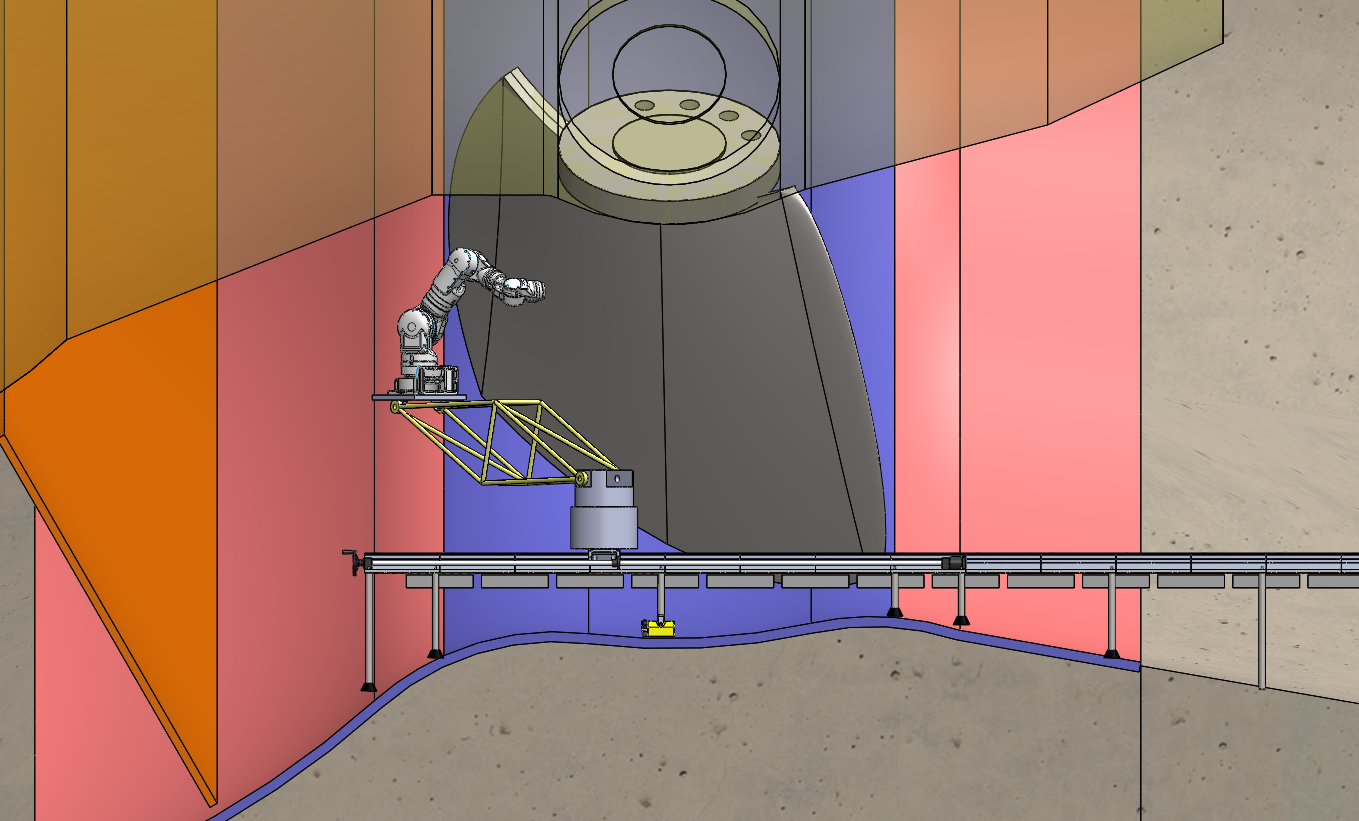
\includegraphics[width=0.8\columnwidth]{figs/bases/base_prr}
   \caption{Base Primático-Rotacional-Rotacional}
   \label{fig::base_prr}
\end{figure}

  A vantagem deste conceito é conferir um alcance grande ao manipulador através
  da base, permitindo que este possa ser de menor alcance próprio, mas ao mesmo
  tempo mais leve.
  Porém, devido à configuração de juntas e pelos resultados encontrados no
  estudo cinemático, a manobrabilidade desta base seria reduzida naquele espaço,
  havendo posicionamentos difíceis de serem alcançados, ou até impossíveis
  dependendo do manipulador escolhido.
  
$\bullet$~\textbf{Base Prismática (P):}

  Este conceito consiste de um trilho (junta prismática) para o transporte do
  manipulador desde a escotilha até o ponto de interesse para revestimento na
  face anterior ou posterior da pá. Quando posicionado, remove-se a seção
  do trilho na direção que obstrui a rotação do rotor. Neste conceito,
  adiciona-se um grau de liberdade ao sistema utilizando a própria rotação do
  rotor, posicionando a pá em relação ao robô. A base mecânica então forneceria
  apenas movimento no trilho na direção do eixo da turbina, deixando fixas as
  outras direções. O procedimento para o revestimento seria o posicionamento do
  rotor, deixando a região a ser processada ao alcance do manipulador; o
  posicionamento do robô no trilho, em relação a pá; a ancoragem do robô
  no ambiente; e o revestimento da região possível para aquela posição.
  Repete-se então este procedimento até ter toda a face processada e
  posiciona-se a próxima pá para revestimento, sem necessidade de mover ou
  desmontar a base do robô até todas as faces daquele lado estarem completas.  A
  figura~\ref{fig::base_p} ilustra este conceito.
  
  \begin{figure}[h!]
   \centering
   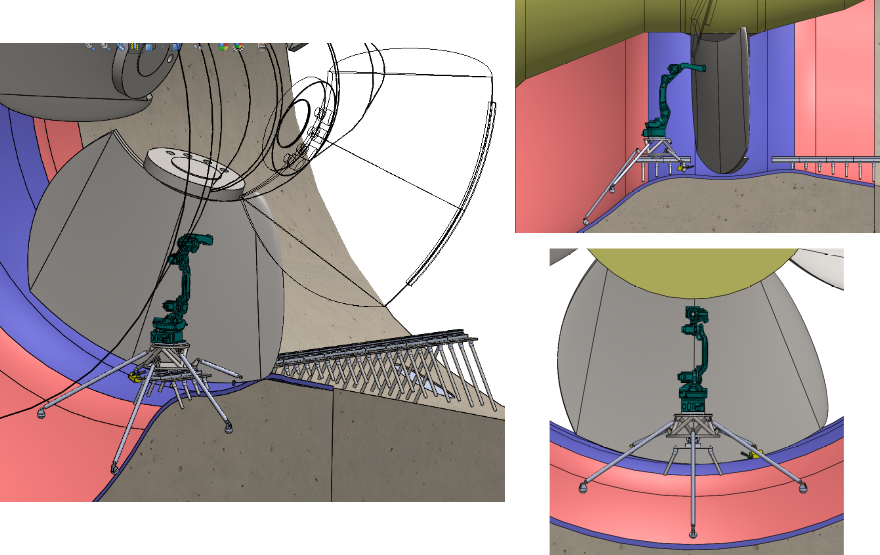
\includegraphics[width=0.8\columnwidth]{figs/bases/base_p}
   \caption{Base Prismática}
   \label{fig::base_p}
\end{figure}
  
  Este conceito foi estudado para o manipulador MH$12$, que de acordo com a
  análise cinemática consegue processar toda a extensão vertical. Para outros
  manipuladores, seria necessário incluir uma junta prismática, adicionando um
  grau de liberdade, na direção vertical.
  
  A análise cinemática também demonstrou que seriam necessárias muitas posições
  do rotor para completar uma face da pá. Há inclusive dificuldades operacionais e
  de segurança no procedimento de rotação do rotor que devem ser considerados. O
  rotor só pode ser girado manualmente, não fornecendo precisão no
  posicionamento da pá em relação a base. Por ser uma tarefa manual, deve-se ter
  procedimentos adequados de segurança para preservar tanto o operador quanto os
  equipamentos próximos. Estas preocupações tornam a solução pouco prática sob o
  ponto de vista operacional.

$\bullet$~\textbf{Base Prismática-Rotacional-Prismática (P-R-P):}

  Este conceito consiste de uma base composta por um trilho primário (junta
  prismática $1$), uma plataforma de base pivotada por mancal e rolamentos entre
  o trilho primário e secundário (junta rotacional) e um trilho secundário
  (junta prismática $2$). Montado o trilho primário alinhado ao eixo da turbina
  a base rotacional sobre o trilho primário, fixa-se o robo sobre a base
  rotacional. Esta base permitrá a montagem do trilho secundário apenas quando o
  robô atingir a região de interesse para revestimento. Quando posicionado o
  manipulador, monta-se então o trilho secundário alinhado ao plano paralelo a
  face da pá e ancora-se a base no ambiente. Desta forma, o robô pode-se
  movimentar ao longo de toda a extensão da pá por meio do trilho secundário e
  também se aproximar e se afastar da superfície da pá, por meio do trilho
  primário. A figura~\ref{fig::base_prp} ilustra este conceito.

\begin{figure}[h!]
   \centering
   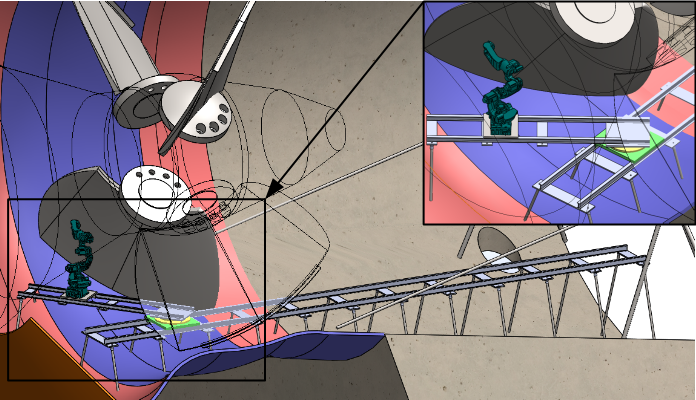
\includegraphics[width=0.9\columnwidth]{figs/bases/base_prp}
   \caption{Base Primática-Rotacional-Prismática}
   \label{fig::base_prp}
\end{figure}

  Desta forma, o rotor deve estar girado em, no mínimo $30^o$ para não haver
  contato com o trilho primário. A análise cinemática será realizada para
  encontrar a melhor configuração de juntas da base que permite ao robô se
  movimentar nos graus de liberdade da base, sem alterar o posicionamento do
  rotor e, assim, cobrir uma face inteira da pá. Para a repetição do processo
  nas outras pás do lado da sucção da turbina, é necessária a desmontagem do
  trilho secundário, o recuo do robô e desmontagem de parte do trilho primário,
  permitindo o giro do rotor para a pá seguinte.
  Para as faces do lado de adução, não é necessária a desmontagem parcial do
  trilho primário.
  
\subsubsection{Sistemas de elevação, fixação e ancoragem}
A entrada de pessoal através da escotilha é feita por uma escada vertical com
guarda-corpo com uma altura total de $5~m$. Equipamentos de segurança como
cinto e talabarte devem ser usados para qualquer um que deseja entrar no
ambiente confinado da turbina, através da escada e isso impossibilita o
transporte manual dos equipamentos. Por este motivo, deve ser instalada uma
estrutura com talha que permita a elevação até o interior da turbina e
movimentação para a áera de montagem adequada. As figuras~\ref{fig::talha} e
\ref{fig::talha_trilho} ilustram a estrutura de elevação com talha e carro
trole. 
  
\begin{figure}[h!]
   \centering
   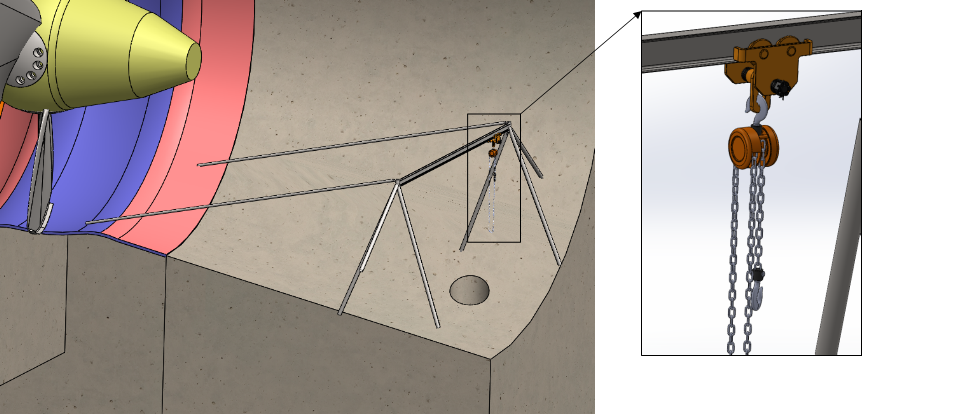
\includegraphics[width=0.8\columnwidth]{figs/bases/talha}
   \caption{Sistema de elevação dos equipamentos}
   \label{fig::talha}
\end{figure}

\begin{figure}[h!]
   \centering
   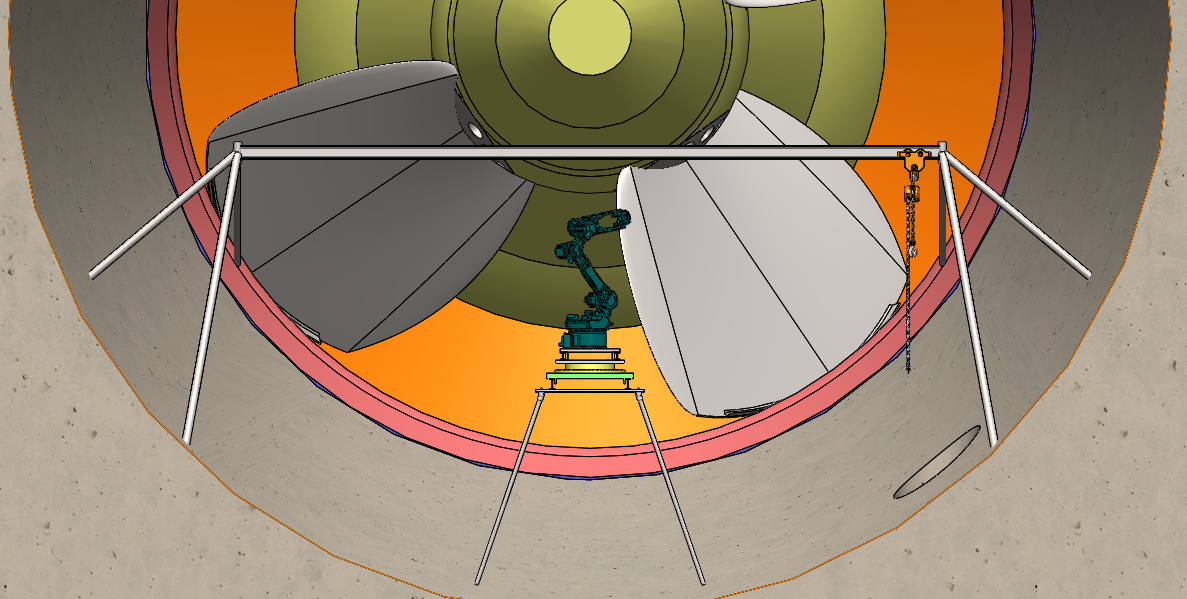
\includegraphics[width=0.8\columnwidth]{figs/bases/talha_trilho}
   \caption{Visão frontal da talha e trilho}
   \label{fig::talha_trilho}
\end{figure}

Devido aos esforços dinâmicos de operação do robô, a fixação da estutura da
base mecânica no ambiente deve ser dimensionada com cuidado. Por se
tratar de um ambiente de escoamento de fluido sob pressão, não são admitidas
modificações permanentes de infra-estrutura no interior da turbina, logo,
qualquer método de fixação utlizado deve ser removível, sem causar nenhum dano
à qualquer superfície. Em visita técnica realizada em Outrubro de $2015$ foi
testada a viabilidade de utlização de bases magnéticas para o sistema de
ancoragem e fixação. Este teste teve o objetivo de verificar a real carga limite de tração
do imã, considerando o ambiente (geometria), materiais e acabamentos
superficiais reais a que estará submetido na solução final. O resultado
detalhado do teste encontra-se no Apêndice~\ref{ape::magnetic}.

Outra opção para fixação provisória seria a soldagem da estrutura na
superfície do túnel. Esta opção segue como uma alternativa ainda para regiões
de difícil fixação da base magnética.
  
\subsubsection{Shutter}%TODO mudar o nome do sistema de desvio do fluxo de
% revestimento
O processo de revestimento HVOF (\textit{High Velocity Oxygen Fuel}) requer
velocidade da pistola controlada de $40~m/min$. Esta velocidade é essencial para
a qualidade do processo e deve ser mantida constante para se obter uma camada 
regular de material ao longo de toda a superfície da peça. Na solução
pesquisada demonstou-se ser inviável utilizar um robô de grande porte, devido a
limitação de acesso e ao confinamento do manipulador no ambiente. Portanto, o
manipulador  escolhido realizará o processo em regiões delimitadas da
superfície da peça e na trajetória haverá inevitavelmente mudanças de direção e
portanto acelerações que irão variar a velocidade da pistola. Durante essas
variações não deve-se injetar o material na peça, sendo necessário um mecanismo
autônomo para impedir o processo nestes intervalos.

A ideia inicialmente estudada foi de uma barreira ao fluxo na saída da pistola. 
A figura~\ref{fig::shutter_todos} ilustra a ideia para dois conceitos nas
configurações aberta e fechada. 
Nestes conceitos, uma barreira é movimentada automaticamente sempre que houver
mudança de direção da pistola, impedindo que o fluxo de material atinja a
pistola. 

\begin{figure}[h!]
   \centering
   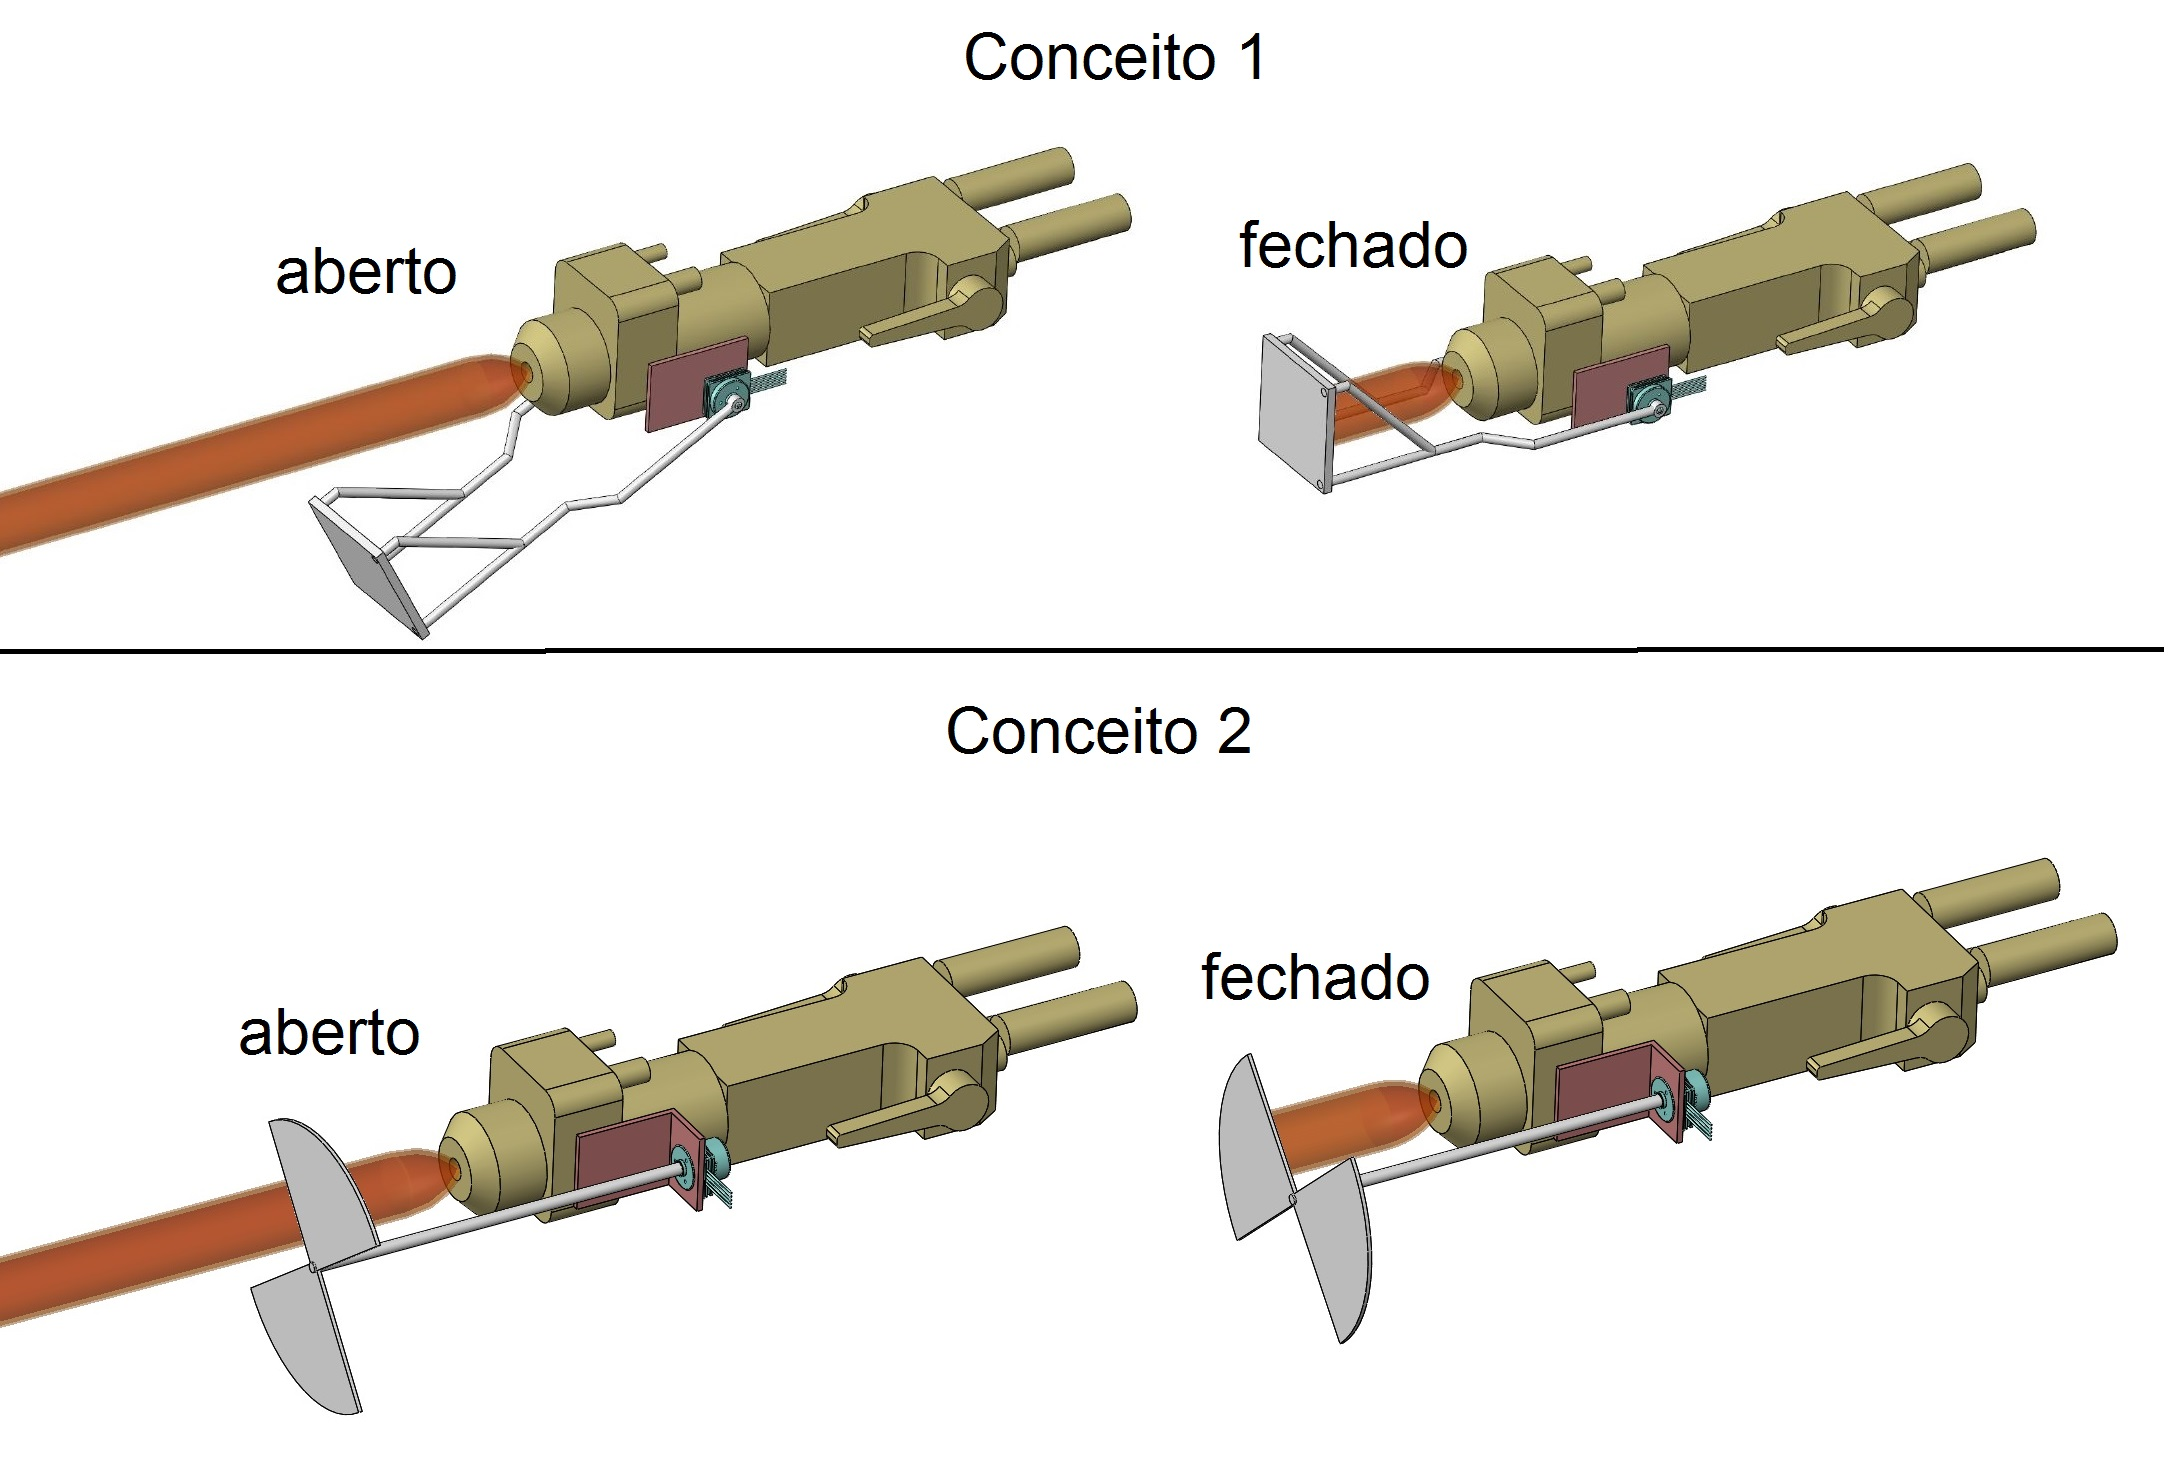
\includegraphics[width=0.8\columnwidth]{figs/shutter/shutter_todos}
   \caption{Conceitos de Shutter avaliados}
   \label{fig::shutter_todos}
\end{figure}

Algumas considerações foram levantadas para avaliar a viabilidade
desta solução, como a alta temperatura da chama, a capacidade do atuador, a
resistência mecânica da barreira e a taxa de acúmulo de material. Este conceito
foi abandonado principalmente devido ao acúmulo de material na barreira, o que
levaria a um aumento de seu peso e por consequência momento de inércia,
alterando a dinâmica prevista ou ainda poderia chegar a obstruir a saída da
chama, causando danos à pistola.

Outra proposta que está sendo estudada é a de modificar o fluxo da linha de
revestimento. A ideia é a inclusão de uma válvula direcional com atuação por
solenóide para desviar o fluxo do material de revestimento para um tanque ou
cilindro de retorno. Esta atuação deve ser autônoma assim como a
trajetória do manipulador. A válvula seria de três vias e duas posições ($3/2$) tal que, no 
repouso, direciona-se o fluxo diretamente para a pistola e, quando
atuada, bloqueia-se o fluxo para a pistola e abre-se o fluxo para exaustão. Uma
válvula limitadora de pressão regulável seria utilizada na linha de exaustão
para igualar as diferenças de pressão entre as duas vias, minimizando efeitos transitórios.
A figura~\ref{fig::circuito_hvof} apresenta o circuito do processo HVOF de forma
simplificada.

 \begin{figure}[h!]
   \centering
   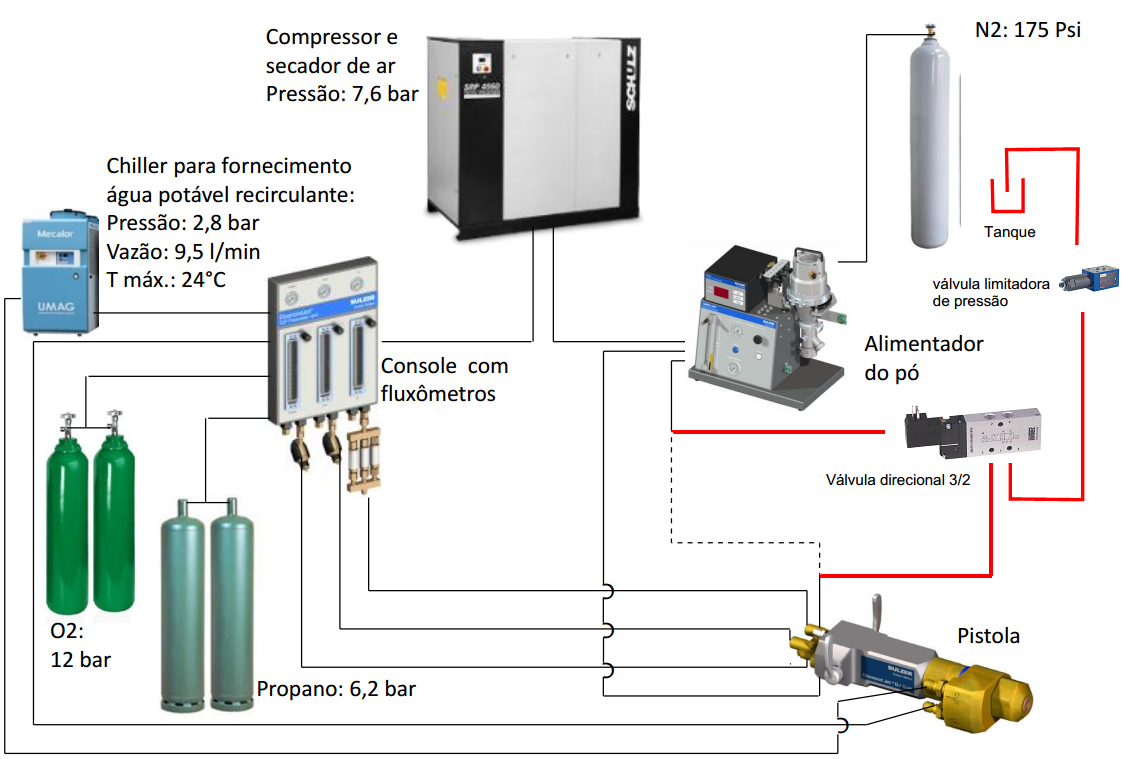
\includegraphics[width=0.8\columnwidth]{figs/shutter/Circuito_HVOF_mod}
   \caption{Circuito do processo HVOF modificado}
   \label{fig::circuito_hvof}
\end{figure}

A linha tracejada representa o circuito original, as linhas em vermelho
representam a modificação do circuito com os equipamentos adicionais indicados.

Esta é uma alternativa que tem como principal vantagem a de poder retornar a
matéria-prima do revestimento para tanque, ou seja, evita-se
o desperdício do material no ambiente. Esta matéria-prima poderia então ser
reaproveitada no processo, separando-se o gás.

%\subsubsection{Soluções de bases mecânicas}
